\section{Data sources and construction}
\label{sec:si-sources}
\subsection{Source inventory and access}
The versioned research-materials repository \citep{gao2026materials} provides source and variable metadata, sample definitions and memberships, and figure--table mappings. The policy-source concordance links corpus identifiers to original documents and coded provisions. These files are organized under \texttt{metadata/} and \texttt{data/}; computational entry points and input access conditions are documented in \texttt{docs/REPRODUCING.md} and \texttt{docs/DATA\_ACCESS.md}.

Table~\ref{tab:data-provenance} records the release, retrieval route, field
coverage and linkage role for every external source.  The charging archive is
the only source of the city--week activity and facility fields; policy,
weather, response-index and geometry inputs are linked at their documented
city, province or coordinate level rather than treated as additional charging
records.
\begingroup\footnotesize\setlength{\tabcolsep}{3pt}\begin{longtable}{@{}>{\raggedright\arraybackslash}p{33mm}>{\raggedright\arraybackslash}p{42mm}>{\raggedright\arraybackslash}p{35mm}>{\raggedright\arraybackslash}p{42mm}@{}}
\caption{Data sources and linkage}\label{tab:data-provenance}\\\toprule
Source / snapshot & Retrieval / file & Coverage / fields & Linkage / use\\\midrule
\endfirsthead\toprule
Source / snapshot & Retrieval / file & Coverage / fields & Linkage / use\\\midrule
\endhead\bottomrule\endfoot
Anonymized operator-network replication archive\par Zenodo v2; 2025-05-31 & \url{https://doi.org/10.5281/zenodo.15564121}\par Replication\_\allowbreak{}AQ\_\allowbreak{}EV.zip /\allowbreak{} Data/\allowbreak{}ev\_\allowbreak{}air.csv & city-week; 2016-2023; 139612 rows\par Total; cumulative\_\allowbreak{}plugs; source city and date & city crosswalk; actual source date\par Charging outcomes and facility-activity comparisons\\[3pt]
Later archive linked by the published Nature Cities article\par Zenodo v3; DOI 10.5281/\allowbreak{}zenodo.17906782 & \url{https://doi.org/10.5281/zenodo.17906782}\par Replication\_\allowbreak{}AQ\_\allowbreak{}EV.zip: README and two .do files & archive version comparison\par README; Table1.do; Table2.do & Not used for the city-week analysis\par Public release scope\\[3pt]
Multi-level energy-transition policy corpus\par Registered figshare v1 & \url{https://doi.org/10.6084/m9.figshare.32182515.v1}\par Registered corpus; gid-indexed policy text & document; local applicability within 2016-2023\par gid; title; authority; publication/\allowbreak{}effective dates; scope; source locator & gid; city identifier; dated administrative applicability\par Policy content, operational obligations and annual associations\\[3pt]
Government policy pages and original-language locators\par Document-specific dates and references & Verified official URLs where available; otherwise the registered corpus record and the versioned \texttt{metadata/}\allowbreak{}\texttt{policy\_sources.csv}\par Government source table and bibliography & document/\allowbreak{}provision\par Title; document number; issuing body; date; article/section/item or descriptive provision; URL status & Document identity and applicable city\par Institutional examples of reporting, maintenance, continuity and payment\\[3pt]
NASA POWER Daily /\allowbreak{} MERRA-2\par API v2.10.1 & \url{https://power.larc.nasa.gov/api/temporal/daily/point}\par POWER daily point API; yearly JSON responses & native grid-day UTC, aggregated city-year; 2016-2023\par T2M; PRECTOTCORR; WS10M; RH2M & Administrative geometry centroid to nearest 0.5 degree latitude x 0.625 degree longitude grid; city identifier/\allowbreak{}year\par Five annual facility controls or four annual policy controls; no quarterly weather\\[3pt]
Oxford COVID-19 Government Response Tracker\par Compact v1; commit e7f66ee39654 & \href{https://raw.githubusercontent.com/OxCGRT/covid-policy-dataset/e7f66ee39654293b5c068efd2f195bd591dc27f6/data/OxCGRT_compact_subnational_v1.csv}{GitHub CSV at the stated commit}\par OxCGRT\_\allowbreak{}compact\_\allowbreak{}subnational\_\allowbreak{}v1.csv & province-day; measured 2020-01-01 to 2023-02-28\par CountryCode; Jurisdiction; RegionCode; Date; StringencyIndex\_\allowbreak{}Average & CountryCode=CHN; Jurisdiction=STATE\_\allowbreak{}TOTAL; 31 explicit province codes; source dates\par Annual policy and paired quarterly response-index comparison ending in 2022\\[3pt]
Administrative geometry in the charging archive\par v2 package; original provider and boundary year not confirmed & \url{https://doi.org/10.5281/zenodo.15564121}\par Map/\allowbreak{}Location/\allowbreak{}ChinaCity.geojson & 372 administrative features; EPSG:4326\par properties.adcode; names; geometry & Unique normalized administrative codes: 333 city matches; unresolved combined name retains no polygon\par Maps and weather city-grid linkage\\[3pt]
\end{longtable}\endgroup


The charging observations come from \texttt{Data/ev\_air.csv} in version 2 of
the anonymized operator-network replication archive (released 31 May 2025;
DOI \url{10.5281/zenodo.15564121}), associated with \citet{ma2026}.  The file
contains 139,612 city-week rows.  \texttt{Total} supplies recorded weekly
activity and \texttt{cumulative\_plugs} supplies the cumulative facility
indicator; the auxiliary summary files are not order-level data.  The archive
snapshot, access route and field-level provenance are listed in the source
inventory \citep{evarchive2025}.

The formal article (DOI \url{10.1038/s44284-026-00395-2}) links a later archive at DOI \url{10.5281/zenodo.17906782}. Version 2 is used here because it supplies the city-week file and geometry required for these comparisons; those inputs are absent from the later archive contents examined for this study. This material choice does not equate the selected release with the formal article's 292-city estimation data. The author plotting code labels activity ``EVCA per station (kWh),'' but the label does not resolve the released activity unit or its zero coding. The facility field likewise has no uniform station, pile or connector definition. All ratios retain the released scales.

The policy input is the registered multi-level energy-transition corpus at
figshare DOI \url{10.6084/m9.figshare.32182515.v1}.  Its document identifiers,
authority, dated local scope and \texttt{gid} values are retained.  The archive
README states that original policy text located through
\url{https://pkulaw.com/} requires an institutional or individual subscription;
the government-source table therefore gives a human-readable provision
reference, a short source-record key and a verified official URL only where one
was checked.  A blank or unverified URL is not replaced by an invented link;
the corresponding corpus identifier and fragment metadata are retained in the
versioned repository source table.  Public corpus availability therefore does
not imply that every source text is freely retrievable through the DOI.

\subsection{Linkage, dates and measurement scale}
The field-to-measure mapping is summarized in Table~\ref{tab:data-dictionary}.
It distinguishes the released activity and facility indicators from the
derived ratios used for descriptive comparisons and models.

The city crosswalk retains original names, standardized city and province
identifiers, and administrative codes.  A valid source date determines the
natural year and calendar quarter.  A compatible week has a valid date and a
positive cumulative facility indicator; source-coded zero activity is retained.
For the compatible dates of city $i$ in period $t$, let $Q_{it}$ denote summed
recorded activity, $E_{it}$ the summed released facility indicator, and
$W_{it}$ the number of compatible weeks.  The derived measures are
\begin{equation}
 A_{it}=Q_{it}/W_{it},\qquad N_{it}=E_{it}/W_{it},\qquad
 I_{it}=Q_{it}/E_{it}.
 \label{eq:si-source-measures}
\end{equation}
The released facility series is used as provided rather than reconstructed from
\texttt{plug\_num}; $W$ counts actual source dates, including 53 weeks in 2017
and 2023.  Duplicate week-number labels do not replace date matching.  A
missing compatible period remains missing, and a source-coded zero is not
reinterpreted as an unobserved outcome.

The same compatibility rule is used for annual and quarterly aggregation, but
the resulting periods serve different analyses.  The descriptive endpoint
windows require only finite endpoint $Q\geq0$, $E>0$ and $W>0$; the annual
models additionally require their stated weather and within-city support, and
the quarterly models join consecutive integer calendar-quarter ordinals.  The
policy comparison uses its own dated-document and source-date support.  These
sets overlap in identifiers but are not one nested estimation sample.

\subsection{Weather, response index and geometry}
NASA POWER Daily requests use the point endpoint and parameters
\texttt{T2M}, \texttt{PRECTOTCORR}, \texttt{WS10M} and \texttt{RH2M}, with
\texttt{community=AG}, \texttt{format=JSON} and
\texttt{time-standard=UTC}; yearly requests span 20160101--20231231.  T2M is
in degrees Celsius, PRECTOTCORR in mm/day, WS10M in m/s, and RH2M in percent;
$-999$ denotes a missing value.  Representative points are
\texttt{geometry.centroid} coordinates from the archived administrative
polygons, matched to the nearest native MERRA-2 grid cell (0.5 degrees
latitude by 0.625 degrees longitude).  They are point-to-grid assignments, not
city-area means.  Annual temperature, wind and humidity means require at least
95\% of the actual 365/366-day calendar.  Precipitation is summed as daily
mm/day times one day and is retained only with a complete calendar, as are
\[
 HDD18=\sum_d\max(18-T_d,0),\qquad
 CDD24=\sum_d\max(T_d-24,0),
\]
measured in degree-days.  Missing annual totals are not annualized.  The
unresolved combined city has no weather coordinate.

\begin{sloppypar}
Pandemic responses use the compact subnational OxCGRT series. The measure is its \texttt{Stringency\allowbreak{}Index\_\allowbreak{}Average} field, from \texttt{OxCGRT\_\allowbreak{}compact\_\allowbreak{}subnational\_\allowbreak{}v1.csv}. Filters
retain \texttt{CountryCode=CHN},
\texttt{Jurisdiction=STATE\_\allowbreak{}TOTAL} and the 31 explicitly matched
province codes.  The codebook defines the compact Average field as the final
average index, weighted where calculable with a simple-average fallback.  Its
measured coverage is 1 January 2020--28 February 2023.  The analysis averages
the index over compatible charging source dates, assigns pre-2020 structural
zeros by rule, and leaves dates outside source coverage missing without forward
filling.  The quarterly comparison ends in 2022 because its estimation support
requires complete exposure; this endpoint is distinct from the source's final
measured date.  The index measures policy responses, not infection prevalence
or total travel disruption.
\end{sloppypar}

The geometry file is \texttt{Map/Location/ChinaCity.geojson} in the charging
archive.  Its 372 features use EPSG:4326.  Normalized administrative-code
matching identifies 333 unique study-city polygons; the combined source name
伊犁哈萨克孜勒苏柯尔克孜 remains in the tabular registry without an assigned
polygon.  Its exclusion affects maps and weather linkage, not the analytical
registry.  The archive metadata do not establish the original boundary provider
or boundary year, so attribution remains to the archived file.


The field definitions in Table~\ref{tab:data-dictionary} are followed by a
role table (Table~\ref{tab:sample-roles}) that keeps the common city registry,
descriptive supports and model supports distinct.  The positive annual,
nonnegative annual, policy and quarterly analyses have different eligibility
conditions rather than successive filters on one panel.  The
descriptive table (Table~\ref{tab:sample-descriptives}) reports the associated
variables on their native scales, including the exposure and response-index
quantities used in the model sections.
\begingroup\footnotesize\setlength{\tabcolsep}{3pt}\begin{longtable}{@{}>{\raggedright\arraybackslash}p{30mm}>{\raggedright\arraybackslash}p{48mm}>{\raggedright\arraybackslash}p{30mm}>{\raggedright\arraybackslash}p{44mm}@{}}
\caption{Measurement definitions}\label{tab:data-dictionary}\\\toprule
Variable / source & Definition & Unit / frequency & Analytical use\\\midrule
\endfirsthead\toprule
Variable / source & Definition & Unit / frequency & Analytical use\\\midrule
\endhead\bottomrule\endfoot
Q\par Total & Sum of activity over compatible source dates & released activity units\par city-year or city-quarter & Descriptive and facility/\allowbreak{}activity models\\[3pt]
E\par cumulative\_\allowbreak{}plugs & Sum of the facility indicator over the same compatible dates & facility-indicator weeks\par city-year or city-quarter & Descriptive and facility/\allowbreak{}activity models\\[3pt]
W\par source date & Number of compatible weeks with valid date and positive facility indicator & weeks\par city-year or city-quarter & Descriptive and facility/\allowbreak{}activity models\\[3pt]
Facility addition observation\par \texttt{facility\_valid\_v7} & True when numeric \texttt{facility\_additions\_analysis} is nonmissing and \texttt{facility\_outcome\_status\_v7} is one of \texttt{observed\_complete}, \texttt{observed\_partial}, \texttt{observed\_zero}, \texttt{observed}, \texttt{complete} or \texttt{partial}; missing, uncovered, pre-entry structural and source-coded-unknown statuses are excluded & 0/1\par city-year & Upstream policy-association support gate; not $E$, $W$ or $N$\\[3pt]
A\par Q/\allowbreak{}W & Mean activity per compatible week & released activity units/\allowbreak{}week\par city-year or city-quarter & Descriptive and facility/\allowbreak{}activity models\\[3pt]
N\par E/\allowbreak{}W & Mean facility indicator, not period additions & facility-indicator units\par city-year or city-quarter & Descriptive and facility/\allowbreak{}activity models\\[3pt]
I\par Q/\allowbreak{}E & Activity per facility exposure; not engineering utilization & activity units/\allowbreak{}facility-indicator week\par city-year or city-quarter & Descriptive and facility/\allowbreak{}activity models\\[3pt]
HDD18\par T2M & Sum max(18-T,0), complete calendar & degree-days\par city-year & Annual facility-activity models\\[3pt]
CDD24\par T2M & Sum max(T-24,0), complete calendar & degree-days\par city-year & Annual facility-activity models\\[3pt]
Temperature\par T2M & Annual daily mean with >=95\% calendar coverage & degrees C\par city-year & Annual policy-association models\\[3pt]
Precipitation\par PRECTOTCORR & Annual sum, complete calendar; no scaling of incomplete years & mm/\allowbreak{}year\par city-year & Annual facility-activity and policy-association models\\[3pt]
Wind\par WS10M & Annual daily mean with >=95\% calendar coverage & m/\allowbreak{}s\par city-year & Annual facility-activity and policy-association models\\[3pt]
Humidity\par RH2M & Annual daily mean with >=95\% calendar coverage & percent\par city-year & Annual facility-activity and policy-association models\\[3pt]
Information/\allowbreak{}supervision $R$ & Information/\allowbreak{}supervision requirement observed by previous year end; unknown coverage distinct from observed absence & 0/\allowbreak{}1 on eligible support\par city-year & Annual policy association\\[3pt]
Operation/\allowbreak{}maintenance $S$ & Operation/\allowbreak{}maintenance requirement observed by previous year end; same coverage rule & 0/\allowbreak{}1 on eligible support\par city-year & Annual policy association\\[3pt]
Previous-year construction support $B$ & Count of documents assigned to the previous year by effective/publication-year rules in Section S3; not cumulative stock & documents\par city-year & Annual policy association\\[3pt]
Response index\par StringencyIndex\_\allowbreak{}Average & Mean on compatible source dates; pre-2020 structural zero; divided by 10 in regression & index points (0-100); regression per 10 points\par province-day to city-year/\allowbreak{}quarter & Annual policy and quarterly paired comparison\\[3pt]
Activity observation state & Compatible source-coded zero retained; no compatible weeks means missing ratios; zero does not certify physical inactivity & categorical\par city-year/\allowbreak{}quarter & All measurements and sample definitions\\[3pt]
\end{longtable}\endgroup

\begingroup\footnotesize\setlength{\tabcolsep}{3pt}\begin{longtable}{@{}>{\raggedright\arraybackslash}p{40mm}>{\raggedright\arraybackslash}p{23mm}>{\raggedright\arraybackslash}p{35mm}>{\raggedright\arraybackslash}p{54mm}@{}}
\caption{Analytical sample roles}\label{tab:sample-roles}\\\toprule
Analytical set & Rows / cities & Period / unit & Purpose\\\midrule
\endfirsthead\toprule
Analytical set & Rows / cities & Period / unit & Purpose\\\midrule
\endhead\bottomrule\endfoot
City registry & 2,672 / 334 & 2016--2023\par city-year & Common observation frame, including unavailable charging outcomes\\[3pt]
Facility-observable city-years & 890 / 293 & 2016--2023\par city-year & Facility distribution and compatible-week availability\\[3pt]
Positive-activity city-years & 464 / 123 & 2016--2023\par city-year & Positive activity/\allowbreak{}intensity distributions\\[3pt]
Continuous 2019-2023 cohort & 180 / 36 & 2019--2023\par city-year & Growth and recorded-week decomposition; positive each year\\[3pt]
Common contribution cities & 208 / 52 & 2020--2023\par city-year in two endpoint pairs & Compare weighted contributions with fixed membership\\[3pt]
Local policy corpus & 601 / 176 & 2016--2023\par documents & Locally applicable policy content\\[3pt]
Documents with requirements & 207 / 88 & 2016--2023\par documents (466 clauses) & Nonexclusive operational responsibility functions\\[3pt]
Annual positive facility model & 445 / 104 & 2016--2023\par city-year & Conditional facility-activity association\\[3pt]
Annual nonnegative facility model & 523 / 112 & 2016--2023\par city-year & Conditional facility-activity association\\[3pt]
Annual policy comparison & 325 / 94 & 2016--2022\par city-year & Recorded R/\allowbreak{}S exposures, with and without response-index adjustment\\[3pt]
Quarterly facility models & 1,542 / 111 & 2017--2023\par city-quarter & Conditional facility-activity association\\[3pt]
Quarterly response-index pair & 1,090 / 94 & 2017--2022\par city-quarter & Facility-activity association with and without response-index adjustment\\[3pt]
\end{longtable}\endgroup

\begingroup\footnotesize\setlength{\tabcolsep}{3pt}\begin{longtable}{@{}>{\raggedright\arraybackslash}p{40mm}>{\raggedright\arraybackslash}p{21mm}>{\raggedright\arraybackslash}p{20mm}>{\raggedright\arraybackslash}p{20mm}>{\raggedright\arraybackslash}p{20mm}>{\raggedright\arraybackslash}p{28mm}@{}}
\caption{Estimation-sample descriptives}\label{tab:sample-descriptives}\\\toprule
Variable (unit) & Valid / missing & Mean & SD & Median & P25--P75\\\midrule
\endfirsthead\toprule
Variable (unit) & Valid / missing & Mean & SD & Median & P25--P75\\\midrule
\endhead\bottomrule\endfoot
\textbf{Annual positive facility model} &  &  &  &  & \\[3pt]
Activity A (source units/\allowbreak{}week) & 445 / 0 & 85,786.50 & 177,294.52 & 8,595.34 & 488.66--56,549.01\\[3pt]
Facilities N (facility units) & 445 / 0 & 293.45 & 672.01 & 50.42 & 19.08--206.00\\[3pt]
Intensity I (source units/\allowbreak{}facility-week) & 445 / 0 & 362.66 & 450.10 & 202.08 & 16.94--551.75\\[3pt]
Compatible weeks W (weeks) & 445 / 0 & 47.27 & 12.18 & 52.00 & 52.00--53.00\\[3pt]
HDD18 (degree-days) & 445 / 0 & 1,698.28 & 1,057.96 & 1,570.19 & 1,175.26--2,125.66\\[3pt]
CDD24 (degree-days) & 445 / 0 & 335.21 & 204.15 & 327.77 & 192.02--453.52\\[3pt]
Precipitation (mm/\allowbreak{}year) & 445 / 0 & 1,329.88 & 491.40 & 1,344.16 & 992.15--1,697.98\\[3pt]
Wind (m/\allowbreak{}s) & 445 / 0 & 3.31 & 0.75 & 3.31 & 2.85--3.73\\[3pt]
Humidity (percent) & 445 / 0 & 74.94 & 9.41 & 78.14 & 71.98--81.16\\[3pt]
\textbf{Annual nonnegative facility model} &  &  &  &  & \\[3pt]
Activity A (source units/\allowbreak{}week) & 523 / 0 & 72,998.89 & 166,346.40 & 4,015.88 & 38.94--46,102.92\\[3pt]
Facilities N (facility units) & 523 / 0 & 252.31 & 627.62 & 37.57 & 12.00--161.76\\[3pt]
Intensity I (source units/\allowbreak{}facility-week) & 523 / 0 & 308.74 & 434.67 & 116.60 & 1.51--494.72\\[3pt]
Compatible weeks W (weeks) & 523 / 0 & 45.71 & 14.36 & 52.00 & 52.00--52.00\\[3pt]
HDD18 (degree-days) & 523 / 0 & 1,774.51 & 1,093.77 & 1,609.76 & 1,215.08--2,336.86\\[3pt]
CDD24 (degree-days) & 523 / 0 & 326.58 & 198.35 & 321.42 & 182.38--438.65\\[3pt]
Precipitation (mm/\allowbreak{}year) & 523 / 0 & 1,313.86 & 501.91 & 1,322.70 & 940.61--1,679.49\\[3pt]
Wind (m/\allowbreak{}s) & 523 / 0 & 3.32 & 0.76 & 3.33 & 2.88--3.73\\[3pt]
Humidity (percent) & 523 / 0 & 74.56 & 9.63 & 77.98 & 70.84--81.14\\[3pt]
\textbf{Annual policy comparison} &  &  &  &  & \\[3pt]
Activity A (source units/\allowbreak{}week) & 325 / 0 & 88,572.91 & 176,259.81 & 11,516.98 & 599.56--63,429.92\\[3pt]
Facilities N (facility units) & 325 / 0 & 265.36 & 592.07 & 44.33 & 17.84--190.98\\[3pt]
Intensity I (source units/\allowbreak{}facility-week) & 325 / 0 & 418.27 & 488.58 & 270.67 & 24.64--646.91\\[3pt]
Compatible weeks W (weeks) & 325 / 0 & 46.01 & 13.23 & 52.00 & 52.00--52.00\\[3pt]
Temperature (degrees C) & 325 / 0 & 16.90 & 3.98 & 16.90 & 15.21--18.31\\[3pt]
Precipitation (mm/\allowbreak{}year) & 325 / 0 & 1,388.66 & 473.78 & 1,409.81 & 1,058.85--1,738.19\\[3pt]
Wind (m/\allowbreak{}s) & 325 / 0 & 3.30 & 0.71 & 3.31 & 2.86--3.69\\[3pt]
Humidity (percent) & 325 / 0 & 75.86 & 8.23 & 78.40 & 73.18--82.07\\[3pt]
R (0/\allowbreak{}1) & 325 / 0 & 0.39 & 0.49 & 0.00 & 0.00--1.00\\[3pt]
S (0/\allowbreak{}1) & 325 / 0 & 0.23 & 0.42 & 0.00 & 0.00--0.00\\[3pt]
Lagged construction count (documents) & 325 / 0 & 0.57 & 1.13 & 0.00 & 0.00--1.00\\[3pt]
Response index (0-100) & 325 / 0 & 35.60 & 26.33 & 49.09 & 0.00--55.53\\[3pt]
\textbf{Quarterly facility models} &  &  &  &  & \\[3pt]
Activity A (source units/\allowbreak{}week) & 1542 / 0 & 96,660.76 & 191,972.42 & 8,748.09 & 210.32--72,772.93\\[3pt]
Facilities N (facility units) & 1542 / 0 & 329.02 & 716.51 & 57.00 & 20.00--236.17\\[3pt]
Intensity I (source units/\allowbreak{}facility-week) & 1542 / 0 & 329.85 & 429.19 & 153.04 & 4.54--526.81\\[3pt]
Compatible weeks W (weeks) & 1542 / 0 & 13.09 & 0.33 & 13.00 & 13.00--13.00\\[3pt]
\textbf{Quarterly response-index pair} &  &  &  &  & \\[3pt]
Activity A (source units/\allowbreak{}week) & 1090 / 0 & 102,545.69 & 194,049.59 & 14,097.61 & 173.98--85,905.90\\[3pt]
Facilities N (facility units) & 1090 / 0 & 302.94 & 641.36 & 52.00 & 17.12--231.12\\[3pt]
Intensity I (source units/\allowbreak{}facility-week) & 1090 / 0 & 382.84 & 467.50 & 214.76 & 6.83--619.12\\[3pt]
Compatible weeks W (weeks) & 1090 / 0 & 13.02 & 0.25 & 13.00 & 13.00--13.00\\[3pt]
Response index (0-100) & 1090 / 0 & 38.91 & 26.09 & 50.66 & 0.00--57.84\\[3pt]
\end{longtable}\endgroup

\FloatBarrier
\section{Descriptive objects and comparisons}
\label{sec:si-descriptive}
\subsection{Observation coverage and fixed-window supports}
Observation states partition the 334-city annual registry (Table~\ref{tab:si_coverage});
analytical memberships overlap because each comparison answers a different
question.  The facility-observable distributions use all compatible records; model
samples impose their own eligibility conditions, while the positive-only
windows require positive activity and facilities in every included year.  The three-year windows thus do
not admit cities observed only at their endpoints.  Baseline-scale groups use
empirical 2022 facility terciles in the 93-city 2022--2023 sample, retaining
identical boundary values together.
\begin{table}[htbp]\centering\small
\caption{Annual observation states}\label{tab:si_coverage}
\begin{tabular}{@{}lrrrr@{}}
\toprule
Year & Facility observed & Positive activity & Coded zero & No compatible weeks \\\midrule
2016 & 18 & 13 & 5 & 316 \\
2017 & 29 & 25 & 4 & 305 \\
2018 & 41 & 36 & 5 & 293 \\
2019 & 47 & 41 & 6 & 287 \\
2020 & 70 & 56 & 14 & 264 \\
2021 & 167 & 81 & 86 & 167 \\
2022 & 225 & 98 & 127 & 109 \\
2023 & 293 & 114 & 179 & 41 \\
\bottomrule\end{tabular}
\end{table}


The coverage table separates a city with a compatible facility observation,
a compatible source-coded-zero activity value and a year with no compatible
weeks.  This distinction is used throughout the endpoint comparisons: a
recorded zero remains an observed value, whereas an absent compatible period
remains missing.  The complete fixed-window changes and regime shares are
reported in the main growth table (Table~\mainref{tab:growth_windows}); the
support table here provides the observation-state context rather than another
growth summary.

The variable-specific quantiles in Table~\ref{tab:si_distributions} use a
strictly positive condition for the variable in that row, not the common
positive-activity model sample.  Thus the $N$ rows have 890 observations in
both scopes because compatibility already requires $N>0$, whereas the
positive-only $A$, $Q$ and $I$ rows contain the 464 positive-activity records.
\begin{table}[htbp]\centering\small
\caption{Facility-observable distributions}\label{tab:si_distributions}
\begin{tabular}{@{}llrrrrrr@{}}
\toprule
Variable & Scope & Rows & P05 & P25 & P50 & P75 & P95 \\\midrule
N & All compatible & 890 & 1.00 & 4.00 & 12.67 & 53.04 & 796.00 \\
N & Positive only & 890 & 1.00 & 4.00 & 12.67 & 53.04 & 796.00 \\
A & All compatible & 890 & 0.00 & 0.00 & 2.02 & 8,527.92 & 313,682.66 \\
A & Positive only & 464 & 3.69 & 454.06 & 6,829.25 & 52,282.63 & 564,777.99 \\
I & All compatible & 890 & 0.00 & 0.00 & 0.13 & 202.65 & 958.48 \\
I & Positive only & 464 & 0.18 & 15.47 & 185.84 & 542.85 & 1,203.74 \\
Q & All compatible & 890 & 0.00 & 0.00 & 61.23 & 358,843.17 & 16,451,166.69 \\
Q & Positive only & 464 & 101.46 & 19,323.68 & 315,775.14 & 2,676,097.51 & 29,450,068.05 \\
W & All compatible & 890 & 7.00 & 42.00 & 52.00 & 53.00 & 53.00 \\
W & Positive only & 890 & 7.00 & 42.00 & 52.00 & 53.00 & 53.00 \\
\bottomrule\end{tabular}
\end{table}


The 2022 facility-scale grouping is summarized in Table~\ref{tab:si_size}.
Figure~\ref{fig:si_spatial} places the same recent-window members in two
views: panel (a) maps the city-level recent $\Delta\ln I$, while panel (b)
uses median markers and P25--P75 intervals for the $A$, $N$ and $I$ changes in
the three equal-sized initial-$N$ groups.  The intensity medians are 0.113,
$-0.078$ and $-0.144$ from low to high initial scale, with intervals
$[-0.855,1.077]$, $[-0.390,0.560]$ and $[-0.481,0.005]$, respectively.  These
P25--P75 values are within-group distribution ranges, not confidence
intervals or formal significance tests.  The medians vary across initial-scale
groups, but within-group variation is substantial; interval overlap or
inclusion of zero is therefore not interpreted as a between-group test.
\begin{table}[htbp]\centering\small
\caption{Facility-scale groups}\label{tab:si_size}
\begin{tabular}{@{}llrrrr@{}}
\toprule
Group & Outcome & Cities & Median & P25 & P75 \\\midrule
Low & A & 31 & 0.630 & -0.324 & 2.583 \\
Low & N & 31 & 0.539 & 0.284 & 1.059 \\
Low & I & 31 & 0.113 & -0.855 & 1.077 \\
Middle & A & 31 & 0.422 & 0.176 & 1.099 \\
Middle & N & 31 & 0.529 & 0.221 & 0.755 \\
Middle & I & 31 & -0.078 & -0.390 & 0.560 \\
High & A & 31 & 0.094 & -0.005 & 0.460 \\
High & N & 31 & 0.331 & 0.204 & 0.544 \\
High & I & 31 & -0.144 & -0.481 & 0.005 \\
\bottomrule\end{tabular}
\end{table}

\begin{figure}[htbp]\centering
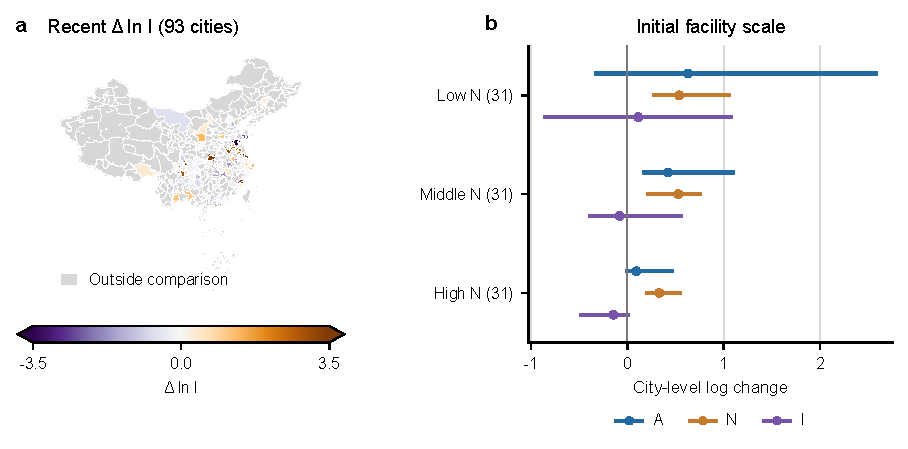
\includegraphics[width=\linewidth,height=.76\textheight,keepaspectratio]{figures/figS_spatial_scale.pdf}
\caption{Recent-window spatial and initial-scale differences}\label{fig:si_spatial}
\end{figure}
\FloatBarrier

The map uses the 95th percentile of the 93 absolute log-intensity changes as a
symmetric colour limit.  Five cities exceed that limit and are shown with
saturated colour and directional markers; their unmodified values are listed
in Table~\ref{tab:map_extremes}.  Grey administrative areas are outside the
comparison, not zero changes.
\begin{table}[htbp]\centering\small
\caption{Extreme city changes}\label{tab:map_extremes}
\begin{tabular}{@{}lrrr@{}}
\toprule
City & Log activity change & Log facility change & Log intensity change \\\midrule
Linyi & -5.943 & 0.984 & -6.927 \\
Meishan & 7.065 & 0.186 & 6.878 \\
Ningde & 7.673 & 1.711 & 5.963 \\
Xiangyang & 4.848 & 0.284 & 4.564 \\
Suining & 4.264 & 0.511 & 3.754 \\
\bottomrule\end{tabular}
\end{table}


\subsection{Recorded activity states and endpoint decomposition}
The four adjacent endpoint comparisons retain a city when both endpoint records
have finite $Q\geq0$, $E>0$, $W>0$ and finite positive $N=E/W$, using the
compatible-week definitions in Section~\ref{sec:si-sources}.  The endpoint
member set is fixed within each window and is not subjected to annual-model
weather, separation or singleton restrictions.  The activity state is $++$
for $Q_0>0,Q_1>0$, $0+$ for $Q_0=0,Q_1>0$, $+0$ for $Q_0>0,Q_1=0$, and $00$
for $Q_0=Q_1=0$.  These are source-record states; missing activity and
source-coded zero remain distinct.

For a fixed window member set $C$, let
$S_{A,t}=\sum_{i\in C}A_{it}$ and $S_{N,t}=\sum_{i\in C}N_{it}$, with
$I^{\mathrm{agg}}_t=S_{A,t}/S_{N,t}$.  The state-group facility share is
$s_{g,t}=\sum_{i\in g}N_{it}/S_{N,t}$, so the four shares sum to one at each
endpoint.  The activity accounting identity is
\begin{equation}
 \Delta S_A=\bigl(S_{A,++,1}-S_{A,++,0}\bigr)
 +S_{A,0+,1}-S_{A,+0,0}+0_{00}.
 \label{eq:si-state-activity}
\end{equation}
Each displayed state contribution is divided by the full-member baseline
$S_{A,0}$ and reported in percentage points, so the terms sum to the full-set
percentage change when that baseline is nonzero.  A zero baseline leaves the
relative change undefined rather than receiving an offset.  The full member
set and its $++$ subset use their own endpoint totals.  The facility levels and
shares are reported in Table~\ref{tab:record_state_details}; the paired
activity and intensity endpoints in Table~\ref{tab:record_state_activity_details}
show how the identity relates state composition to aggregate changes.  These
details complement the complete recorded-state endpoint aggregates in the
main observation table (Table~\mainref{tab:recorded_states}).
\begingroup\scriptsize\setlength{\tabcolsep}{3pt}\begin{longtable}{@{}llrrrrrr@{}}\caption{Recorded-state facility levels and shares}\label{tab:record_state_details}\\\toprule
Window & State & Cities & City share (\%) & $N_0$ & $N_1$ & $N_0$ share (\%) & $N_1$ share (\%)\\
\midrule\endfirsthead\toprule
Window & State & Cities & City share (\%) & $N_0$ & $N_1$ & $N_0$ share (\%) & $N_1$ share (\%)\\
\midrule\endhead\bottomrule\endfoot
2019--2020 & All members & 47 & 100.0 & 9,458.07 & 12,854.31 & 100.0 & 100.0\\
2019--2020 & ++ & 39 & 83.0 & 9,400.07 & 12,788.69 & 99.4 & 99.5\\
2019--2020 & 0+ & 3 & 6.4 & 23.00 & 30.62 & 0.2 & 0.2\\
2019--2020 & +0 & 2 & 4.3 & 26.00 & 26.00 & 0.3 & 0.2\\
2019--2020 & 00 & 3 & 6.4 & 9.00 & 9.00 & 0.1 & 0.1\\
2020--2021 & All members & 70 & 100.0 & 13,919.80 & 20,423.21 & 100.0 & 100.0\\
2020--2021 & ++ & 55 & 78.6 & 13,826.23 & 20,259.67 & 99.3 & 99.2\\
2020--2021 & 0+ & 5 & 7.1 & 38.00 & 104.62 & 0.3 & 0.5\\
2020--2021 & +0 & 1 & 1.4 & 10.00 & 10.79 & 0.1 & 0.1\\
2020--2021 & 00 & 9 & 12.9 & 45.57 & 48.13 & 0.3 & 0.2\\
2021--2022 & All members & 167 & 100.0 & 21,365.20 & 31,041.77 & 100.0 & 100.0\\
2021--2022 & ++ & 77 & 46.1 & 20,861.79 & 30,273.98 & 97.6 & 97.5\\
2021--2022 & 0+ & 11 & 6.6 & 45.51 & 123.90 & 0.2 & 0.4\\
2021--2022 & +0 & 4 & 2.4 & 43.63 & 79.60 & 0.2 & 0.3\\
2021--2022 & 00 & 75 & 44.9 & 414.26 & 564.29 & 1.9 & 1.8\\
2022--2023 & All members & 225 & 100.0 & 31,453.75 & 45,829.57 & 100.0 & 100.0\\
2022--2023 & ++ & 93 & 41.3 & 30,504.65 & 43,555.91 & 97.0 & 95.0\\
2022--2023 & 0+ & 10 & 4.4 & 100.63 & 482.75 & 0.3 & 1.1\\
2022--2023 & +0 & 5 & 2.2 & 117.21 & 198.49 & 0.4 & 0.4\\
2022--2023 & 00 & 117 & 52.0 & 731.25 & 1,592.42 & 2.3 & 3.5\\
\end{longtable}
\medskip\begin{longtable}{@{}llrrrrrr@{}}\caption{Recorded-state activity and intensity endpoints}\label{tab:record_state_activity_details}\\\toprule
Window & State & $A_0$ & $A_1$ & $\Delta A$ (\%) & $I_0$ & $I_1$ & $\Delta I$ (\%)\\
\midrule\endfirsthead\toprule
Window & State & $A_0$ & $A_1$ & $\Delta A$ (\%) & $I_0$ & $I_1$ & $\Delta I$ (\%)\\
\midrule\endhead\bottomrule\endfoot
2019--2020 & All members & 4,837,522.3 & 5,208,395.8 & 7.67 & 511.47 & 405.19 & -20.78\\
2019--2020 & ++ & 4,836,773.6 & 5,205,037.1 & 7.61 & 514.55 & 407.00 & -20.90\\
2019--2020 & 0+ & 0.0 & 3,358.7 & -- & 0.00 & 109.71 & --\\
2019--2020 & +0 & 748.7 & 0.0 & -100.00 & 28.80 & 0.00 & -100.00\\
2019--2020 & 00 & 0.0 & 0.0 & -- & 0.00 & 0.00 & --\\
2020--2021 & All members & 5,238,049.8 & 7,585,617.2 & 44.82 & 376.30 & 371.42 & -1.30\\
2020--2021 & ++ & 5,233,362.2 & 7,582,463.4 & 44.89 & 378.51 & 374.26 & -1.12\\
2020--2021 & 0+ & 0.0 & 3,153.9 & -- & 0.00 & 30.15 & --\\
2020--2021 & +0 & 4,687.6 & 0.0 & -100.00 & 468.76 & 0.00 & -100.00\\
2020--2021 & 00 & 0.0 & 0.0 & -- & 0.00 & 0.00 & --\\
2021--2022 & All members & 7,732,921.9 & 8,029,944.0 & 3.84 & 361.94 & 258.68 & -28.53\\
2021--2022 & ++ & 7,730,386.8 & 8,017,728.8 & 3.72 & 370.55 & 264.84 & -28.53\\
2021--2022 & 0+ & 0.0 & 12,215.2 & -- & 0.00 & 98.59 & --\\
2021--2022 & +0 & 2,535.1 & 0.0 & -100.00 & 58.10 & 0.00 & -100.00\\
2021--2022 & 00 & 0.0 & 0.0 & -- & 0.00 & 0.00 & --\\
2022--2023 & All members & 8,107,848.9 & 9,350,117.5 & 15.32 & 257.77 & 204.02 & -20.85\\
2022--2023 & ++ & 8,107,584.8 & 9,316,257.5 & 14.91 & 265.78 & 213.89 & -19.52\\
2022--2023 & 0+ & 0.0 & 33,859.9 & -- & 0.00 & 70.14 & --\\
2022--2023 & +0 & 264.1 & 0.0 & -100.00 & 2.25 & 0.00 & -100.00\\
2022--2023 & 00 & 0.0 & 0.0 & -- & 0.00 & 0.00 & --\\
\end{longtable}\endgroup


\subsection{Growth regimes, transitions and network contributions}
For the positive-only windows, $x_i=\ln(N_{i1}/N_{i0})$,
$y_i=\ln(A_{i1}/A_{i0})$ and $dI_i=y_i-x_i$.  The three principal categories
are facility expansion with faster activity growth ($x_i>0,y_i>x_i$),
expansion with slower positive activity growth ($x_i>0,0<y_i<x_i$), and
expansion with activity contraction ($x_i>0,y_i<0$).  Facility nonexpansion,
exact ties and other boundary cases remain separate.  A tolerance of
$10^{-10}$ is used only for floating-point equality at zero or $y=x$.  All
city--window members are retained, and repeated cities across windows are not
independent observations.

The main fixed-window table gives the aggregate changes and category shares
(Table~\mainref{tab:growth_windows}).  The detailed transition table contains
both the 52-city 2020--2021 to 2022--2023 comparison and the 73-city
2021--2022 to 2022--2023 comparison (Table~\ref{tab:growth_transition_details});
the second comparison shares 2022 and therefore describes paired
classifications rather than an independent sample.  Early categories are
columns and late categories rows.  For cell $(r,c)$,
$100n_{rc}/\sum_{r'}n_{r'c}$ is the conditional percentage; empty early
categories have no denominator.  ``Other'' retains its subtypes and is not an
ordered growth level; those subtypes are listed separately in
Table~\ref{tab:growth_transition_other}.  In the 73-city comparison, 32 pairs
retain the same category (43.84\%); six of 23 early faster-growth cities move
to slower-positive growth, five of 25 early slower-positive cities move to
faster growth, and 7 of 14 early contraction cities move to positive late
growth.  These percentages use their respective early-category denominators.
\begin{table}[htbp]\centering\small\setlength{\tabcolsep}{4pt}\caption{Within-city growth-regime transitions}\label{tab:growth_transition_details}
\begin{tabular}{@{}lrrrrr@{}}\toprule
\multicolumn{6}{l}{52-city comparison: 2020--2021 to 2022--2023}\\\midrule
Late / early & Faster & Slower & Contraction & Other & Late total\\
Faster & 10 (37.0) & 0 (0.0) & 1 (33.3) & 4 (40.0) & 15\\
Slower & 10 (37.0) & 8 (66.7) & 2 (66.7) & 0 (0.0) & 20\\
Contraction & 7 (25.9) & 3 (25.0) & 0 (0.0) & 5 (50.0) & 15\\
Other & 0 (0.0) & 1 (8.3) & 0 (0.0) & 1 (10.0) & 2\\
Early total & 27 & 12 & 3 & 10 & 52\\
\midrule
\multicolumn{6}{l}{73-city comparison: 2021--2022 to 2022--2023}\\\midrule
Late / early & Faster & Slower & Contraction & Other & Late total\\
Faster & 10 (43.5) & 5 (20.0) & 3 (21.4) & 3 (27.3) & 21\\
Slower & 6 (26.1) & 15 (60.0) & 4 (28.6) & 1 (9.1) & 26\\
Contraction & 7 (30.4) & 5 (20.0) & 6 (42.9) & 6 (54.5) & 24\\
Other & 0 (0.0) & 0 (0.0) & 1 (7.1) & 1 (9.1) & 2\\
Early total & 23 & 25 & 14 & 11 & 73\\
\midrule
\bottomrule\end{tabular}\end{table}\FloatBarrier
\begingroup\scriptsize\setlength{\tabcolsep}{3pt}\begin{longtable}{@{}p{42mm}llr@{}}\caption{Other growth-regime subtypes}\label{tab:growth_transition_other}\\\toprule
Comparison & Period & Other subtype & Cities\\
\midrule\endfirsthead\toprule
Comparison & Period & Other subtype & Cities\\
\midrule\endhead\bottomrule\endfoot
52-city comparison: 2020--2021 to 2022--2023 & Early & Facility unchanged; activity contraction & 2\\
52-city comparison: 2020--2021 to 2022--2023 & Early & Facility unchanged; activity increase & 8\\
52-city comparison: 2020--2021 to 2022--2023 & Late & Facility unchanged; activity contraction & 1\\
52-city comparison: 2020--2021 to 2022--2023 & Late & Facility unchanged; activity increase & 1\\
73-city comparison: 2021--2022 to 2022--2023 & Early & Facility unchanged; activity contraction & 4\\
73-city comparison: 2021--2022 to 2022--2023 & Early & Facility unchanged; activity increase & 7\\
73-city comparison: 2021--2022 to 2022--2023 & Late & Facility unchanged; activity contraction & 1\\
73-city comparison: 2021--2022 to 2022--2023 & Late & Facility unchanged; activity increase & 1\\
\end{longtable}\endgroup

\clearpage
\begin{figure}[htbp]\centering
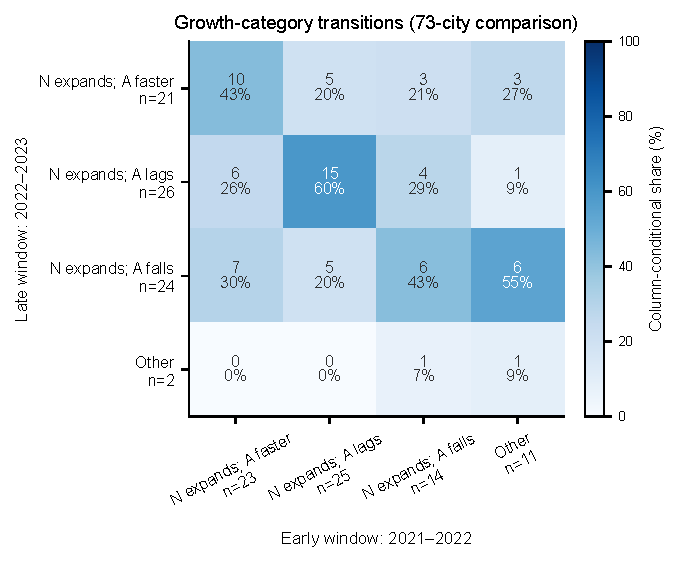
\includegraphics[width=\linewidth]{figures/growth_transitions_supplement.pdf}
\caption{Growth regime transitions, supplementary comparison}\label{fig:si_growth_transitions}
\end{figure}
\FloatBarrier
Figure~\ref{fig:si_growth_transitions} visualizes the column-conditional
73-city matrix, making the persistence of the slower-positive category and the
reclassification of early contraction cases readable without treating the
categories as an ordered process.  The primary non-overlapping transition
comparison is shown in the main transition figure (Figure~\mainref{fig:transitions}).

For the network contribution analysis, city contributions are expressed in
index points relative to each window's initial aggregate intensity of 100.
Within-city and facility-weight components are evaluated separately; a change
in facility share can therefore make the weighted contribution differ in sign
from the city's own intensity change.  The complete main-text decomposition is
reported in Table~\mainref{tab:contributions} and Figure~\mainref{fig:contributions}.
The detailed component rows in Table~\ref{tab:si_contributions} retain all
windows, sign differences and top-five absolute shares, while
Table~\ref{tab:si_concentration} reports HHI and top-negative-contribution
concentration using the stated fixed supports.  Concentration uses either total
absolute net contributions or all negative net contributions as its denominator,
not the net decline.  The largest-five and largest-fifth summaries use the
corresponding fixed support; the 52-city comparison retains the same members at
both windows.
\begin{table}[htbp]\centering\small
\caption{Detailed network contributions}\label{tab:si_contributions}
\begin{tabular}{@{}lrrrrr@{}}
\toprule
Window & Within & Weights & Net & Top 5 abs. (\%) & Signs differ\\\midrule
2019--2023 & -61.321 & 6.466 & -54.855 & 62.78 & 6\\
2019--2020 & -25.068 & 4.167 & -20.901 & 64.20 & 6\\
2020--2021 & -6.160 & 5.038 & -1.122 & 49.98 & 15\\
2021--2022 & -26.098 & -2.431 & -28.529 & 49.63 & 15\\
2022--2023 & -21.666 & 2.142 & -19.524 & 38.91 & 15\\
2019--2021 & -29.040 & 7.886 & -21.154 & 70.42 & 8\\
2020--2022 & -31.732 & 1.825 & -29.907 & 58.90 & 10\\
2021--2023 & -42.302 & -0.068 & -42.370 & 46.90 & 12\\
\bottomrule\end{tabular}
\end{table}

\begin{table}[htbp]\centering\setlength{\tabcolsep}{4pt}\small
\caption{Negative-contribution concentration}\label{tab:si_concentration}
\begin{tabular}{@{}lrrrrrl@{}}\toprule
Window & Cities & $m$ & HHI & Norm. HHI & Top 5 (\%) & Top 20\%: $k$, share\\\midrule
2019--2023 & 36 & 28 & 0.144 & 0.113 & 65.62 & 6: 71.63\\
2019--2020 & 39 & 26 & 0.231 & 0.200 & 74.36 & 6: 78.25\\
2020--2021 & 55 & 24 & 0.181 & 0.145 & 76.24 & 5: 76.24\\
2021--2022 & 77 & 44 & 0.078 & 0.057 & 52.79 & 9: 75.11\\
2022--2023 & 93 & 49 & 0.068 & 0.048 & 45.24 & 10: 76.49\\
2019--2021 & 38 & 24 & 0.259 & 0.227 & 80.63 & 5: 80.63\\
2020--2022 & 53 & 28 & 0.116 & 0.083 & 64.60 & 6: 70.30\\
2021--2023 & 73 & 43 & 0.076 & 0.054 & 50.55 & 9: 75.56\\
2020--2021 & 52 & 22 & 0.184 & 0.145 & 76.92 & 5: 76.92\\
2022--2023 & 52 & 36 & 0.071 & 0.044 & 46.46 & 8: 68.40\\
\bottomrule\end{tabular}
\end{table}

\FloatBarrier

\subsection{Recorded-week composition}
The record-structure analysis keeps the exact city membership of the five-year
and latest-year windows and compares their endpoints.  At an endpoint with
nonnegative compatible-week activity and at least one positive week, let $p$ be
the fraction of compatible weeks with positive recorded activity and $q^+$ the
mean activity among those positive weeks.  Then
\begin{equation}
 A=pq^+,\qquad I=\frac{pq^+}{N},\qquad
 \Delta\ln I=\Delta\ln p+\Delta\ln q^+-\Delta\ln N.
 \label{eq:si-recording-composition}
\end{equation}
The identity is evaluated for the fixed 36-city 2019--2023 and 93-city
2022--2023 memberships.  Equal-city mean log components satisfy the identity;
medians are reported independently and are not treated as an additive
decomposition.  The calculation requires complete records and at least one
positive week for each city-endpoint; zero, missing and negative-record
diagnostics remain in the endpoint table.  Compatible-week coverage divides
observed compatible weeks by calendar source-week exposure and uses the same
members as the component decomposition.  Table~\ref{tab:observation} gives the
component changes, while Figure~\ref{fig:si_recording_coverage} separates
compatible-week coverage from source-coded-zero weeks.  These panels support
the distinction between observation structure and the activity or intensity
ratios summarized in the main recording figure (Figure~\mainref{fig:recording}).
\begin{table}[htbp]\centering\small
\caption{Recorded activity components}\label{tab:observation}
\begin{tabular}{@{}lp{.34\linewidth}rrrr@{}}
\toprule
Window & Component & Mean & Median & P25 & P75 \\\midrule
2019--2023 & Positive-record proportion & 0.202 & 0.000 & 0.000 & 0.005 \\
2019--2023 & Positive-week mean activity & 0.749 & 0.561 & 0.107 & 0.965 \\
2019--2023 & Facilities & 1.538 & 1.316 & 0.854 & 2.063 \\
2019--2023 & Intensity & -0.587 & -0.585 & -1.192 & -0.242 \\
2022--2023 & Positive-record proportion & 0.201 & 0.000 & 0.000 & 0.039 \\
2022--2023 & Positive-week mean activity & 0.605 & 0.297 & -0.001 & 1.064 \\
2022--2023 & Facilities & 0.634 & 0.474 & 0.239 & 0.808 \\
2022--2023 & Intensity & 0.171 & -0.083 & -0.494 & 0.409 \\
\bottomrule\end{tabular}
\end{table}

\begin{figure}[htbp]\centering
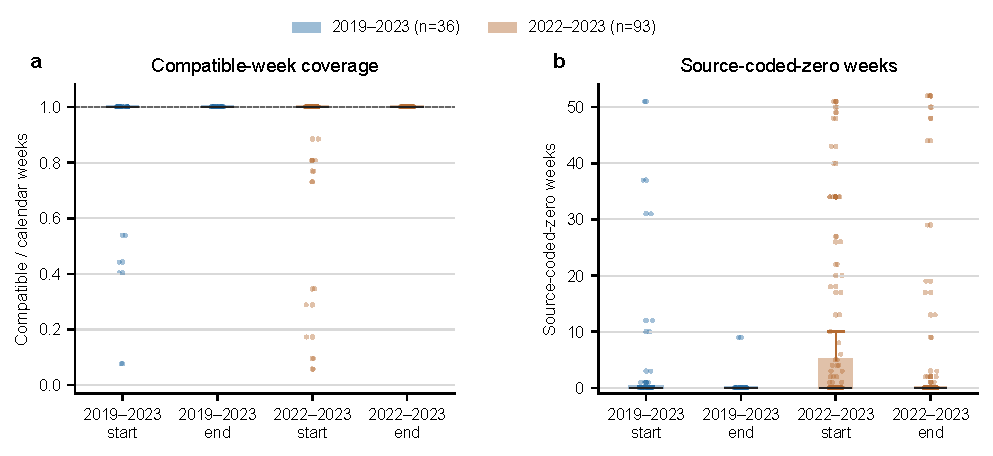
\includegraphics[width=\linewidth]{figures/figS_recording_coverage.pdf}
\caption{Observation coverage and coded-zero weeks}\label{fig:si_recording_coverage}
\end{figure}
\FloatBarrier

\section{Policy coding and timing}
\label{sec:si-policy}
\subsection{Policy content coding}
\label{sec:si-policy-methods}

The policy evidence is represented at three linked levels: clause, document
and city.  The research-window corpus contains 601 locally applicable
documents covering 176 cities.  Of these, 207 documents covering 88 cities
contain 466 retained requirement clauses.  A document enters the analytical
content corpus when it has a local administrative scope, an applicable date
within the study frame, and a requirement or condition that can be linked to
charging infrastructure or its operation.  A clause is the classification
unit; document and city identifiers are retained separately and are not
additive counts.  Original language, translated wording, document identity,
source locator, publication date, effective date and date precision are
retained for every evidence record.

The codebook records four functional groups: information and supervision;
operation and maintenance; continuing operation or payment; and assessable or
subsidy-linked conditions.  A label describes what a text requires, monitors
or conditions.  It is not a measure of compliance, policy intensity or realized
service.  Labels are non-exclusive: a clause may require both reporting and
maintenance, or condition payment on continued operation.  Functional city
counts therefore overlap and cannot be summed to a policy total.  Evidence is
located by the retained source fragment, document identifier and
clause identifier.  Because labels are non-exclusive, the functional counts
describe the number of clauses meeting each requirement definition rather than
a partition of documents or cities.

\subsection{Governance timing registry}
The timing registry is separate from the 88-city content scope and contains 95
cities with a qualifying governance record.  Construction support is coded
$B$, information or supervision $R$, and operating-service responsibility
$S$; $G$ denotes the combined path following the first qualifying $R$ or $S$
requirement.  Here $B$ identifies construction-support events; the annual
regressor $B_{i,t-1}$ defined below is a prior-year document count.
Publication and effective dates are retained separately.  For
each record, let $[a,b]$ be the inclusive interval implied by the earliest known
lower bound and latest known upper bound at the reported precision.  A calendar
quarter is clean pre-policy only when its end precedes $a$, transitional when it
intersects $[a,b]$, and fully post-policy only when its start follows $b$.
Year-only dates remain intervals and are not assigned an artificial event
quarter.  Unknown coverage or unresolved timing remains unknown and is not
coded as untreated.  A first year with observed facilities is not interpreted
as a construction or commissioning date.

The timing table retains the city-level dates, precision, pre-period support and
first/second-year availability needed by the governance comparison.  Content
coverage, governance timing, charging observations and their intersections
remain separate denominators in the accompanying overlap tables.  This keeps a
documented responsibility distinct from the later quarterly support and from
the annual association estimand.

\subsection{Annual construction-support year assignment}
For the annual policy count $B$, a document is assigned to a calendar year only
when its effective year is known.  When both effective and publication years are
known, the assigned year is the later of the two; when the effective year is
known but the publication year is not, the effective year is used.  When the
effective year is unknown, the assigned year remains unknown even if a
publication year is available.  The annual regressor $B_{i,t-1}$ is the number
of qualifying construction-support policy documents assigned to the preceding
calendar year $t-1$; it is a prior-year document count, not a cumulative stock.
The $R$ and $S$ indicators are already defined at the end of the preceding year
and are not lagged a second time.  This year-assignment rule is distinct from
the quarterly date-interval rule above: a quarter is cleanly pre-policy only
when its end precedes the lower bound, transitional when it intersects the
interval, and fully post-policy only when its start follows the upper bound.


The functional coverage counts in Table~\ref{tab:si_policy_landscape} are
clause, document and city counts with nonexclusive labels.  The policy--outcome
overlap in Table~\ref{tab:si_overlap} keeps separate denominators for content
functions, the governance registry and charging observations; it is a support
description, not a policy-effect comparison.
\begin{table}[htbp]\centering\small
\caption{Policy function coverage}\label{tab:si_policy_landscape}
\begin{tabular}{@{}p{.57\linewidth}rrr@{}}
\toprule
Function & Clauses & Documents & Cities \\\midrule
information and supervision & 284 & 168 & 78 \\
operation and maintenance & 97 & 58 & 35 \\
continuous operation and payment & 15 & 11 & 11 \\
measurable or subsidy-linked conditions & 47 & 33 & 19 \\
unclassified retained attributes & 80 & 52 & 29 \\
\bottomrule\end{tabular}
\end{table}

\begin{table}[htbp]\centering\small
\caption{Policy--outcome coverage}\label{tab:si_overlap}
\begin{tabular}{@{}p{.34\linewidth}rrrrr@{}}
\toprule
Scope & Policy & Facilities & Positive & Long 36 & Recent 93\\\midrule
All retained content & 88 & 87 & 49 & 21 & 41\\
Information / supervision & 78 & 77 & 43 & 19 & 35\\
Operation / maintenance & 35 & 35 & 24 & 12 & 22\\
Continuity / payment & 11 & 11 & 9 & 5 & 9\\
Assessable / subsidy-linked & 19 & 19 & 14 & 5 & 12\\
Unclassified attributes & 29 & 28 & 21 & 12 & 17\\
Governance registry & 95 & 94 & 55 & 23 & 46\\
\bottomrule\end{tabular}
\end{table}


The function definitions and city reach are illustrated in
Table~\ref{tab:policy_functions}, and the retained source excerpts in
Table~\ref{tab:policy} show how requirements are assigned to those functions.
The main policy-sequence figure (Figure~\mainref{fig:policy}) provides the
compact overview; the SI tables preserve the full coding and source context.
\begin{table}[htbp]\centering\small
\caption{Policy functions}\label{tab:policy_functions}
\begin{tabular}{@{}p{.23\linewidth}p{.37\linewidth}p{.31\linewidth}@{}}
\toprule
Function / city reach & Documented example & Object for evaluation\\\midrule
Information and supervision (78/88) & Suzhou: real-time safety monitoring of public charging facilities \citep{gov12}. & Platform connection, data transmission and accessible monitoring records.\\
Operation and maintenance (35/88) & Haikou: service guarantees during holidays, including operation and maintenance \citep{gov7}. & Equipment condition, maintenance response and service provision during specified periods.\\
Continuing operation or payment (11/88) & Dongguan: continued-operation commitment for new applicants and remaining subsidy after a year of normal operation \citep{gov1}. & Duration of operation and evidence supporting a subsequent payment.\\
Assessable or subsidy-linked (19/88) & Dongguan: eligibility and staged disbursement conditions in the construction subsidy \citep{gov1}. & Observable eligibility, acceptance and operating conditions tied to support.\\
\bottomrule\end{tabular}
\end{table}

\begin{table}[htbp]\centering\small
\caption{Policy examples}\label{tab:policy}
\begin{tabularx}{\linewidth}{@{}p{.16\linewidth}X p{.38\linewidth}@{}}\toprule
City/source & Original wording and translation & Policy reference and provision \\\midrule
Wuhan \citep{gov5}\newline \href{https://github.com/DS-Gao/ev-charging-service-dynamics/blob/v1.0.0/metadata/policy_sources.csv}{Corpus record: P005} & 重点解决充电运营企业之间信息、支付等环节的不兼容问题 \newline \emph{Resolve incompatibility in information and payment between charging operators.} & Section II(3), information/payment interoperability in charging infrastructure; Section II(4), monitoring platform; \href{https://www.wuhan.gov.cn/zwgk/xxgk/zfgb/202003/P020171106560912432935.pdf}{official PDF} \\
Shaoxing \citep{gov11}\newline \href{https://github.com/DS-Gao/ev-charging-service-dynamics/blob/v1.0.0/metadata/policy_sources.csv}{Corpus record: P011} & 解决充电基础设施资源利用不足问题 \newline \emph{Address insufficient use of charging-infrastructure resources.} & Section II(1), item 4, resource-use demonstration; \href{https://zjjcmspublic.oss-cn-hangzhou-zwynet-d01-a.internet.cloud.zj.gov.cn/jcms_files/jcms1/web2247/site/attach/0/feb5d86c42944dc980ae2feda02c6c79.pdf}{official PDF} \\
Shaoxing \citep{gov11}\newline \href{https://github.com/DS-Gao/ev-charging-service-dynamics/blob/v1.0.0/metadata/policy_sources.csv}{Corpus record: P011} & 规范非充电车占位现象 \newline \emph{Regulate occupation of charging spaces by non-charging vehicles.} & Section II(2), item 8, parking-space occupation and facility utilization; \href{https://zjjcmspublic.oss-cn-hangzhou-zwynet-d01-a.internet.cloud.zj.gov.cn/jcms_files/jcms1/web2247/site/attach/0/feb5d86c42944dc980ae2feda02c6c79.pdf}{official PDF} \\
Dongguan \citep{gov1}\newline \href{https://github.com/DS-Gao/ev-charging-service-dynamics/blob/v1.0.0/metadata/policy_sources.csv}{Corpus record: P001} & 其余资金待充电设施正常运行一年后全额拨付 \newline \emph{Pay the remainder after one year of normal operation.} & Article 15, staged construction-subsidy payment \\
Suzhou \citep{gov12}\newline \href{https://github.com/DS-Gao/ev-charging-service-dynamics/blob/v1.0.0/metadata/policy_sources.csv}{Corpus record: P012} & 对建设运营的公共领域充电设施安全状态进行实时监控 \newline \emph{Monitor the safety status of public charging facilities in real time.} & Section I(2), enterprise monitoring platform and public-facility safety monitoring \\
\bottomrule\end{tabularx}
\end{table}

\FloatBarrier

The document-level provenance, reader-facing provision references and source
record keys are retained in Table~\ref{tab:government_sources}; the versioned
source-to-record mapping is provided in the research-materials repository's
\href{https://github.com/DS-Gao/ev-charging-service-dynamics/blob/v1.0.0/metadata/policy_sources.csv}{\texttt{metadata/policy\_sources.csv}}.
The separate timing registry in
Table~\ref{tab:si_governance_support} provides the dated governance support,
precision and pre-period availability used in the later comparison.  Its
denominator is distinct from both the 88-city content scope and the
charging-observation supports.
\begingroup\setlength{\tabcolsep}{2pt}\begin{longtable}{@{}p{.12\linewidth}p{.48\linewidth}p{.35\linewidth}@{}}
\caption{Government source records}\label{tab:government_sources}\\
\toprule
City/source & Original institution/title and English title & Policy reference and provision \\\midrule
\endfirsthead
City/source & Original institution/title and English title & Policy reference and provision \\\midrule\endhead
Dongguan \citep{gov1} & 东莞市发展和改革局 东莞市发展和改革局关于印发《东莞市发展和改革局新能源汽车推广应用资金管理办法(2019年修订)》的通知\newline Notification of the Dongguan Municipal Development and Reform Bureau on Issuing the Measures for Administration of Funds for the Promotion and Application of New-Energy Vehicles (2019 Revision)\newline 东发改〔2019〕448号 & \href{https://github.com/DS-Gao/ev-charging-service-dynamics/blob/v1.0.0/metadata/policy_sources.csv}{Corpus record: P001}; Article 15, construction-subsidy eligibility and staged payment. \\
Wuhan \citep{gov5} & 武汉市人民政府 武汉市人民政府关于印发武汉市新能源汽车推广应用和产业化工作实施方案(2017—2020年)的通知\newline Notification of the Wuhan Municipal People's Government on Issuing the Implementation Plan for the Promotion and Application and Industrialization of New-Energy Vehicles in Wuhan (2017–2020)\newline 武政规〔2017〕42号 & \href{https://github.com/DS-Gao/ev-charging-service-dynamics/blob/v1.0.0/metadata/policy_sources.csv}{Corpus record: P005}; Section II(3), information/payment interoperability in charging infrastructure, and Section II(4), the monitoring platform. \href{https://www.wuhan.gov.cn/zwgk/xxgk/zfgb/202003/P020171106560912432935.pdf}{Official PDF}. \\
Haikou \citep{gov7} & 海口市发展和改革委员会 海口市发展和改革委员会关于切实做好节假日期间新能源汽车充电服务保障有关工作的函\newline Letter of the Haikou Municipal Development and Reform Commission on Effectively Ensuring New-Energy Vehicle Charging Services During Holidays\newline 海发改体改函〔2023〕434号 & \href{https://github.com/DS-Gao/ev-charging-service-dynamics/blob/v1.0.0/metadata/policy_sources.csv}{Corpus record: P007}; Section II, holiday charging-service safety and operations checks. \\
Shaoxing \citep{gov11} & 绍兴市人民政府办公室 绍兴市人民政府办公室关于印发《绍兴市新能源汽车下乡行动方案(2023—2025年)》《绍兴市完善高质量充电基础设施网络体系实施方案(2023—2025年)》的通知\newline Notification of the General Office of the Shaoxing Municipal People's Government on Issuing the Shaoxing Action Plan for New-Energy Vehicles Going to the Countryside (2023–2025) and the Implementation Plan for Improving the High-Quality Charging Infrastructure Network System in Shaoxing (2023–2025)\newline 绍政办发〔2023〕31号 & \href{https://github.com/DS-Gao/ev-charging-service-dynamics/blob/v1.0.0/metadata/policy_sources.csv}{Corpus record: P011}; Section II(1), item 4, resource-use demonstration, and Section II(2), item 8, parking-space occupation and facility utilization. \href{https://zjjcmspublic.oss-cn-hangzhou-zwynet-d01-a.internet.cloud.zj.gov.cn/jcms_files/jcms1/web2247/site/attach/0/feb5d86c42944dc980ae2feda02c6c79.pdf}{Official PDF}. \\
Suzhou \citep{gov12} & 苏州市经济和信息化委员会 苏州市经济和信息化委员会关于做好新能源汽车推广应用安全监管工作的通知\newline Notification of the Suzhou Municipal Commission of Economy and Information Technology on Strengthening Safety Supervision of New-Energy Vehicle Promotion and Application\newline 苏经信产投〔2017〕2号 & \href{https://github.com/DS-Gao/ev-charging-service-dynamics/blob/v1.0.0/metadata/policy_sources.csv}{Corpus record: P012}; Section I(2), enterprise monitoring platform and public-facility safety monitoring. \\
\bottomrule
\end{longtable}\endgroup

\begingroup\small\renewcommand{\arraystretch}{1.04}
\begin{longtable}{@{}llrrlrrr@{}}
\caption{Governance-date support}\label{tab:si_governance_support}\\
\toprule
City & Code & B year & G year & Precision & Pre n & E/L n & Change \\\midrule
\endfirsthead
City & Code & B year & G year & Precision & Pre n & E/L n & Change \\\midrule\endhead
Sanya & 460200 & 2016 & 2016 & day & 0 & 0/0 & NA \\
Sanming & 350400 & 2016 & 2016 & day & 0 & 0/0 & NA \\
Shanghai & 310000 & 2009 & 2016 & year & 0 & 0/0 & NA \\
Shangrao & 361100 & 2014 & 2014 & day & 0 & 0/0 & NA \\
Dongguan & 441900 & 2012 & 2019 & day & 7 & 3/4 & 4.60 \\
Dongying & 370500 & 2021 & 2021 & day & 0 & 0/0 & NA \\
Zhongwei & 640500 & 2016 & 2023 & day & 8 & 4/4 & 0.42 \\
Linfen & 141000 & 2015 & 2015 & day & 0 & 0/0 & NA \\
Lishui & 331100 & 2016 & 2016 & day & 0 & 0/0 & NA \\
Lijiang & 530700 & 2019 & 2019 & day & 0 & 0/0 & NA \\
Yunfu & 445300 & 2018 & 2018 & day & 0 & 0/0 & NA \\
Foshan & 440600 & 2013 & 2019 & year & 4 & 0/0 & NA \\
Baoding & 130600 & 2017 & 2017 & day & 0 & 0/0 & NA \\
Baoshan & 530500 & 2017 & 2018 & day & 0 & 0/0 & NA \\
Xinyang & 411500 & 2016 & 2018 & day & 0 & 0/0 & NA \\
Karamay & 650200 & 2018 & 2018 & day & 0 & 0/0 & NA \\
Liupanshui & 520200 & 2015 & 2017 & day & 0 & 0/0 & NA \\
Lanzhou & 620100 & 2014 & 2023 & day & 7 & 3/4 & 3.40 \\
Beijing & 110000 & 2011 & 2015 & day & 0 & 0/0 & NA \\
Beihai & 450500 & 2023 & 2023 & day & 6 & 2/4 & 0.00 \\
Nanjing & 320100 & 2014 & 2015 & day & 0 & 0/0 & NA \\
Nanping & 350700 & 2015 & 2017 & day & 0 & 0/0 & NA \\
Nantong & 320600 & 2013 & 2015 & day & 0 & 0/0 & NA \\
Xiamen & 350200 & 2014 & 2017 & day & 5 & 1/4 & NA \\
Taizhou & 331000 & 2016 & 2023 & day & 13 & 4/4 & 35.17 \\
Hefei & 340100 & 2012 & 2012 & day & 0 & 0/0 & NA \\
Zhoukou & 411600 & 2016 & 2016 & day & 0 & 0/0 & NA \\
Shangqiu & 411400 & 2016 & 2021 & day & 0 & 0/0 & NA \\
Tacheng & 654200 & 2022 & 2022 & day & 1 & 0/1 & NA \\
Tianjin & 120000 & 2016 & 2016 & day & 0 & 0/0 & NA \\
Taiyuan & 140100 & 2014 & 2014 & day & 0 & 0/0 & NA \\
Ningde & 350900 & 2015 & 2017 & day & 0 & 0/0 & NA \\
Ningbo & 330200 & 2014 & 2015 & day & 0 & 0/0 & NA \\
Anyang & 410500 & 2016 & 2017 & day & 0 & 0/0 & NA \\
Yichun & 360900 & 2015 & 2023 & day & 9 & 4/4 & 5.96 \\
Suqian & 321300 & 2015 & 2015 & day & 0 & 0/0 & NA \\
Changzhou & 320400 & 2014 & 2015 & day & 0 & 0/0 & NA \\
Pingliang & 620800 & 2016 & 2016 & day & 0 & 0/0 & NA \\
Guangzhou & 440100 & 2014 & 2015 & year & 0 & 0/0 & NA \\
Qingyang & 621000 & 2016 & 2016 & day & 0 & 0/0 & NA \\
Xuzhou & 320300 & 2015 & 2015 & day & 0 & 0/0 & NA \\
Xinzhou & 140900 & 2014 & 2014 & day & 0 & 0/0 & NA \\
Chengdu & 510100 & 2015 & 2020 & day & 11 & 4/4 & 144.25 \\
Yangzhou & 321000 & 2014 & 2015 & day & 0 & 0/0 & NA \\
Jieyang & 445200 & 2018 & 2018 & day & 0 & 0/0 & NA \\
Xinxiang & 410700 & 2014 & 2022 & day & 0 & 0/0 & NA \\
Wuxi & 320200 & 2015 & 2016 & day & 0 & 0/0 & NA \\
Kunming & 530100 & 2015 & 2015 & day & 0 & 0/0 & NA \\
Puer & 530800 & 2018 & 2018 & day & 0 & 0/0 & NA \\
Qujing & 530300 & 2018 & 2018 & day & 0 & 0/0 & NA \\
Hangzhou & 330100 & 2016 & 2016 & day & 1 & 0/1 & NA \\
Liuzhou & 450200 & 2019 & 2020 & day & 0 & 0/0 & NA \\
Meizhou & 441400 & 2017 & 2017 & day & 0 & 0/0 & NA \\
Wuhan & 420100 & 2014 & 2017 & day & 5 & 1/4 & NA \\
Shanwei & 441500 & 2017 & 2017 & day & 0 & 0/0 & NA \\
Jiangmen & 440700 & 2019 & 2019 & day & 0 & 0/0 & NA \\
Shenyang & 210100 & 2015 & 2018 & day & 0 & 0/0 & NA \\
Taian & 370900 & 2010 & 2016 & day & 0 & 0/0 & NA \\
Taizhou & 321200 & 2015 & 2015 & day & 0 & 0/0 & NA \\
Luzhou & 510500 & 2015 & 2015 & day & 0 & 0/0 & NA \\
Luoyang & 410300 & 2018 & 2019 & day & 0 & 0/0 & NA \\
Jinan & 370100 & 2011 & 2020 & day & 0 & 0/0 & NA \\
Haikou & 460100 & 2010 & 2023 & day & 19 & 4/4 & 402.75 \\
Zibo & 370300 & 2022 & 2022 & day & 1 & 0/1 & NA \\
Huaian & 320800 & 2016 & 2016 & day & 0 & 0/0 & NA \\
Shenzhen & 440300 & 2009 & 2015 & day & 0 & 0/0 & NA \\
Wenzhou & 330300 & 2017 & 2022 & day & 13 & 4/4 & 36.79 \\
Huzhou & 330500 & 2014 & 2020 & day & 16 & 4/4 & 0.00 \\
Yantai & 370600 & 2022 & 2022 & day & 5 & 1/4 & NA \\
Jiaozuo & 410800 & 2016 & 2023 & day & 2 & 0/2 & NA \\
Zhuhai & 440400 & 2011 & 2019 & day & 0 & 0/0 & NA \\
Yancheng & 320900 & 2014 & 2020 & day & 0 & 0/0 & NA \\
Fuzhou & 350100 & 2015 & 2017 & day & 5 & 1/4 & NA \\
Shaoxing & 330600 & 2014 & 2023 & day & 22 & 4/4 & 143.67 \\
Zhaoqing & 441200 & 2019 & 2019 & day & 0 & 0/0 & NA \\
Suzhou & 320500 & 2017 & 2017 & day & 2 & 0/2 & NA \\
Putian & 350300 & 2015 & 2017 & day & 0 & 0/0 & NA \\
Quzhou & 330800 & 2020 & 2022 & day & 2 & 0/2 & NA \\
Xiangyang & 420600 & 2009 & 2019 & day & 0 & 0/0 & NA \\
Xian & 610100 & 2013 & 2014 & day & 0 & 0/0 & NA \\
Xuchang & 411000 & 2016 & 2016 & day & 0 & 0/0 & NA \\
Guigang & 450800 & 2020 & 2020 & day & 0 & 0/0 & NA \\
Hezhou & 451100 & 2021 & 2021 & day & 0 & 0/0 & NA \\
Lianyungang & 320700 & 2015 & 2017 & day & 0 & 0/0 & NA \\
Zhengzhou & 410100 & 2011 & 2016 & day & 0 & 0/0 & NA \\
Jiuquan & 620900 & 2020 & 2020 & day & 0 & 0/0 & NA \\
Chongqing & 500000 & 2014 & 2016 & day & 0 & 0/0 & NA \\
Jinhua & 330700 & 2011 & 2023 & day & 17 & 4/4 & 250.67 \\
Yinchuan & 640100 & 2016 & 2016 & day & 0 & 0/0 & NA \\
Zhenjiang & 321100 & 2015 & 2015 & day & 0 & 0/0 & NA \\
Changchun & 220100 & 2011 & 2014 & day & 0 & 0/0 & NA \\
Changzhi & 140400 & 2016 & 2016 & day & 0 & 0/0 & NA \\
Yangjiang & 441700 & 2019 & 2019 & day & 0 & 0/0 & NA \\
Qingdao & 370200 & 2014 & 2023 & day & 12 & 4/4 & 290.69 \\
Zhumadian & 411700 & 2016 & 2019 & day & 0 & 0/0 & NA \\
\bottomrule\end{longtable}

\endgroup

\FloatBarrier

\section{Annual models and inference}
\label{sec:si-annual}
The staged annual eligibility and fixed-effect support exclusions are given in
Table~\ref{tab:sample_models}; this table makes explicit why the positive and
zero-inclusive PPML specifications do not share one row set.
\begin{table}[htbp]\centering\small
\caption{Annual model samples}\label{tab:sample_models}
\begin{tabular}{@{}p{.27\linewidth}rrp{.47\linewidth}@{}}
\toprule
Stage & Rows & Cities & Condition \\\midrule
Positive eligible & 464 & 123 & Positive activity, facilities and compatible weeks \\
Positive estimation & 445 & 104 & Exclude 19 singleton cities \\
Nonnegative eligible & 887 & 292 & Complete annual weather; 423 coded-zero rows \\
After all-zero exclusion & 534 & 123 & Exclude 169 cities and 353 rows \\
Nonnegative estimation & 523 & 112 & Exclude 11 singletons; 453 positive, 70 coded zeros \\
\bottomrule\end{tabular}
\end{table}

\subsection{Annual estimands and sample supports}
\label{sec:si-annual-models}

The annual analysis distinguishes recorded activity from facility exposure.  For
city $i$ and year $t$, let $Q_{it}$ be recorded charging activity, $E_{it}$
the cumulative facility indicator summed over the same compatible weeks, and
$W_{it}$ the number of compatible weeks.  The source-defined measures are
\begin{equation}
 A_{it}=Q_{it}/W_{it},\qquad N_{it}=E_{it}/W_{it},\qquad
 I_{it}=Q_{it}/E_{it}=A_{it}/N_{it},\qquad x_{it}=\log N_{it}.
 \label{eq:si-definitions}
\end{equation}
Compatibility requires a valid source date and positive facilities.  A
source-coded zero activity is retained, whereas a city-year with no compatible
weeks is missing and is not assigned a zero.  Thus $A$ is activity per
compatible week, $N$ is time-average facility exposure, and $I$ is activity per
cumulative facility exposure.  These ratios do not recover latent demand,
instantaneous online capacity or a complete operator total.

The annual sample and its exclusions are shown in Table~\ref{tab:sample_models}.
Before fixed-effect support exclusions, the positive-support sample contains
464 $Q>0$, $E>0$, $W>0$ rows from 123 cities over 2016--2023.  Nineteen
cities contribute exactly one positive year; those rows provide no within-city
information for a city fixed-effect slope and are excluded from the positive
models, leaving 445 rows in 104 cities.  The zero-inclusive support begins
with 887 rows from 292 cities with finite nonnegative $Q$, positive $E$ and
$W$, positive finite $N$, and complete annual weather controls.  It excludes
169 cities (353 rows) whose support-wide activity sum is zero and then 11
singleton cities (11 rows), leaving 523 rows from 112 cities: 453 positive
rows and 70 source-coded-zero rows.  These are support definitions, not
imputations of an unobserved outcome.

\subsection{Conditional means and model specifications}
For the log outcome, the constant-elasticity specification is
\begin{equation}
 \operatorname{E}[\log A_{it}\mid X_{it}]
 =\alpha_i+\lambda_t+\beta x_{it}+\gamma^{\top}Z_{it},
 \label{eq:si-log-l0}
\end{equation}
and a restricted-cubic extension adds two nonlinear terms:
\begin{equation}
 \operatorname{E}[\log A_{it}\mid X_{it}]
 =\alpha_i+\lambda_t+\beta x_{it}+
 \theta_1H_1(x_{it})+\theta_2H_2(x_{it})+\gamma^{\top}Z_{it}.
 \label{eq:si-log-models}
\end{equation}
Here $\alpha_i$ and $\lambda_t$ are city and calendar-year fixed effects.  The
vector $Z_{it}$ contains annual HDD18, CDD24, precipitation, mean wind speed
and mean relative humidity.  These aggregates adjust for measured annual
background conditions; they do not make facility growth exogenous or provide an
instrument.

The level models have a different estimand and retain observation exposure:
\begin{equation}
 \operatorname{E}[Q_{it}\mid X_{it},W_{it}]
 =W_{it}\exp\!\left(\alpha_i+\lambda_t+\beta x_{it}
 +\gamma^{\top}Z_{it}\right),
 \label{eq:si-p0}
\end{equation}
and
\begin{equation}
 \operatorname{E}[Q_{it}\mid X_{it},W_{it}]
 =W_{it}\exp\!\left(\alpha_i+\lambda_t+\beta x_{it}
 +\theta_1H_1(x_{it})+\theta_2H_2(x_{it})
 +\gamma^{\top}Z_{it}\right).
 \label{eq:si-p1}
\end{equation}
The two level equations use Poisson pseudo-maximum likelihood (PPML), whose
estimand is the conditional arithmetic mean of nonnegative $Q$; integer
outcomes and equidispersion are not required.  The positive-support level
equations use the common 445-row positive support, whereas the zero-inclusive
level equation uses the separate 523-row support.  A zero outcome in the zero-inclusive sample is a
source-coded zero under the stated compatibility and weather rules; unknown
activity is never treated as zero.  Panels (a) and (b) of
Figure~\ref{fig:si_annual} use the 445-row, 104-city positive-support fits;
panel (c) additionally compares the positive-support and zero-inclusive
constant PPML estimates.  The two models therefore do not estimate a single
relation in which missingness and a recorded zero are interchangeable.

The offset is $\log W_{it}$ in the PPML linear predictor, not an additional
frequency-weight argument.  If $\mu_{it}$ denotes the modeled weekly mean and
$X_{it}$ is a design row, then
\begin{equation}
 \operatorname{E}[Q_{it}\mid X_{it},W_{it}]=W_{it}\mu_{it},\qquad
 X_{it}(Q_{it}-W_{it}\mu_{it})
 =W_{it}X_{it}(A_{it}-\mu_{it}).
 \label{eq:si-offset-equivalence}
\end{equation}
Compatible-week exposure therefore changes the modeled mean and the
score/information; the absence of a frequency weight does not imply equal
regression influence.  The PPML coefficient is interpreted on the conditional
arithmetic-mean scale, not as an OLS coefficient for a log-transformed
outcome.

\subsection{Restricted-cubic form and local elasticity}
The log and level specifications use the same two-term restricted-cubic basis.
Let $k_1<k_2<k_3<k_4$ be the empirical 0.05, 0.35, 0.65 and 0.95 quantiles of
$x$ in the 445-row positive sample.  Linear quantile interpolation gives the following display-rounded values
\[
(k_1,k_2,k_3,k_4)=(1.0986,\ 3.3273,\ 4.7236,\ 7.3771).
\]
With $(u)_+=\max(u,0)$,
\begin{equation}
 H_j(x)=\frac{(x-k_j)_+^3-
 \dfrac{k_4-k_j}{k_4-k_3}(x-k_3)_+^3+
 \dfrac{k_3-k_j}{k_4-k_3}(x-k_4)_+^3}
 {(k_4-k_1)^2},\qquad j\in\{1,2\}.
 \label{eq:si-rcs}
\end{equation}
The analytic derivative used for local elasticity is
\begin{equation}
 H'_j(x)=\frac{3(x-k_j)_+^2-
 3\dfrac{k_4-k_j}{k_4-k_3}(x-k_3)_+^2+
 3\dfrac{k_3-k_j}{k_4-k_3}(x-k_4)_+^2}
 {(k_4-k_1)^2}.
 \label{eq:si-rcs-derivative}
\end{equation}
For either fitted log mean, the local elasticity is
$\eta(x)=\beta+\theta_1H'_1(x)+\theta_2H'_2(x)$.  It is the local derivative
of the stated conditional function, not an estimated threshold or optimal
stock.  Curve intervals are pointwise city-cluster intervals; no simultaneous
band is claimed.  The joint restrictions remain model-specific: for the
nonlinear log specification, Wald $=2.701$, $F(2,103)=1.351$ and
$p=\LogSplineP$; for the nonlinear level specification, Wald $=3.021$,
$F(2,103)=1.510$ and $p=\MeanSplineP$.  A non-rejection concerns the two
added basis terms on that model's own outcome scale; it is not a global
linearity test or an equality test across models.

\subsection{Clustered inference and contrasts}
For OLS, city-clustered CR1 inference uses the full design rank:
\begin{equation}
 \widehat V_{\mathrm{CR1}}=
 \frac{G}{G-1}\frac{n-1}{n-r}
 (X^\top X)^{-1}
 \left[\sum_{g=1}^{G}X_g^\top\hat u_g\hat u_g^\top X_g\right]
 (X^\top X)^{-1}.
 \label{eq:si-cr1-ols}
\end{equation}
Here $r$ is the actual matrix rank.  The PPML sandwich uses the Poisson
Hessian $X^\top\operatorname{diag}(\hat\mu)X$ and city-summed scores
$X_i(Q_i-\hat\mu_i)$.  The positive sample has rank 117 for the linear log and
positive-support level models and rank 119 for their nonlinear extensions, with
$n=445$, $G=104$, CR1 factors 1.3668 and 1.3752, and $t(G-1)=t(103)$
intervals.  The zero-inclusive level model has rank 125, $G=112$ and
$t(111)$ intervals.  For a local elasticity, if $d(x)$ contains
$1,H'_1(x),H'_2(x)$ in the relevant scale-coefficient positions, its variance
is $d(x)'\widehat Vd(x)$ and its pointwise interval is
\[
 \hat\eta(x)\mathbin{\pm}t_{G-1,.975}\sqrt{d(x)'\widehat Vd(x)}.
\]
The joint test uses $F=(\theta'V_\theta^{-1}\theta)/2$ with its
model-specific covariance block.  These conditional intervals address
within-city dependence, not sample selection or policy endogeneity.
The main annual table (Table~\mainref{tab:annual_models}) reports the three
constant-elasticity estimates, their $\beta-1$ contrasts and the corresponding
tests against zero and one.  The rank, cluster degrees of freedom and
covariance construction above supply the inference details for those reported
contrasts, with each test remaining on its model's stated conditional-mean scale.


The joint tests of the two added restricted-cubic terms are reported in
Table~\ref{tab:nonlinear_tests}.  The test is model-specific: a non-rejection
does not establish global linearity or equality between the log and level
models.
\begin{table}[htbp]\centering\small
\caption{Nonlinear association tests}\label{tab:nonlinear_tests}
\begin{tabular}{@{}llrrr@{}}
\toprule
Model & Restrictions & F statistic & df & p \\\midrule
Log-OLS spline & 2 & 1.350518 & 2, 103 & 0.263655 \\
PPML spline & 2 & 1.510305 & 2, 103 & 0.225692 \\
\bottomrule\end{tabular}
\end{table}

\begin{figure}[htbp]\centering
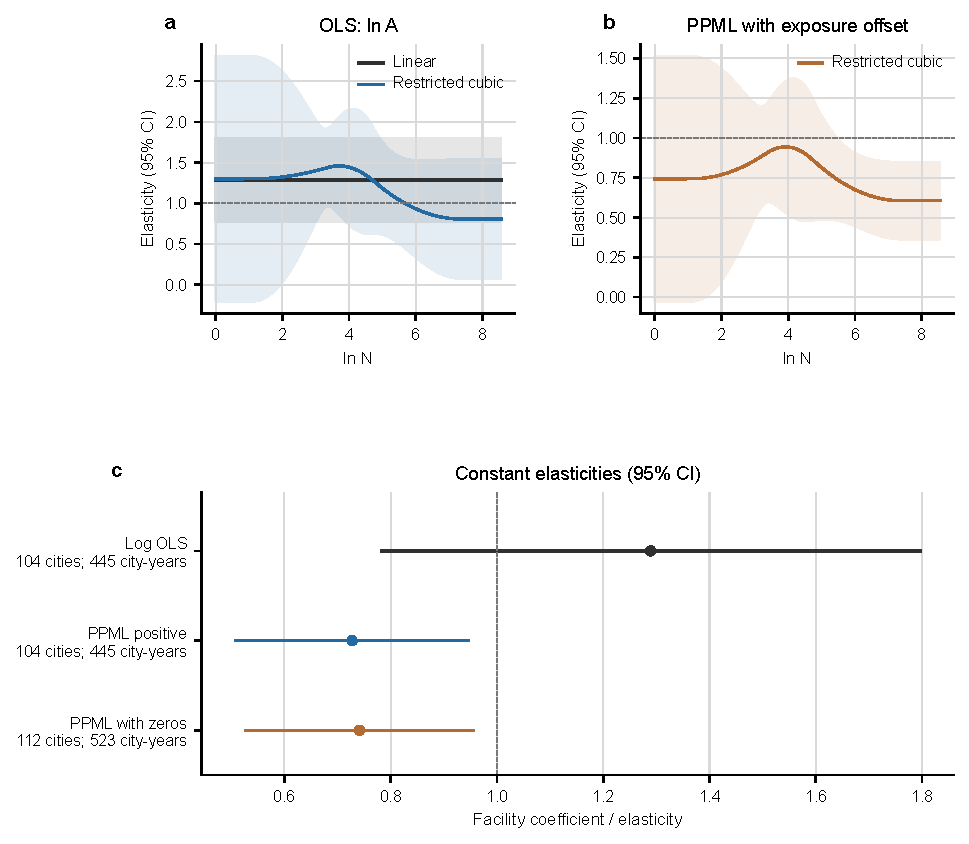
\includegraphics[width=\linewidth]{figures/figS_annual_models.pdf}
\caption{Annual conditional elasticities by model}\label{fig:si_annual}
\end{figure}
\FloatBarrier
Figure~\ref{fig:si_annual} shows local elasticity over $\ln N$ on each model's
own outcome scale: the OLS curve is for conditional log activity, whereas the
PPML curve is for the conditional arithmetic mean with the exposure offset.
The constant estimates are placed together for direct coefficient comparison,
while the curves retain pointwise 95\% intervals over facility scale.  In the
constant specifications, the positive-support and zero-inclusive PPML
estimates are 0.727 $[0.509,0.946]$ and 0.741 $[0.528,0.955]$, respectively,
whereas the OLS estimate is 1.289 $[0.783,1.796]$; the PPML intervals lie below
one while the OLS interval includes one.  These are different conditional mean
objects, so the scale-specific curves and their uncertainty are interpreted
within model rather than as a single common elasticity.  The complete
coefficients and tests against zero and unit elasticity are in Table~\mainref{tab:annual_models}.

\section{Quarterly facility--activity dynamics}
\label{sec:si-quarterly}
\subsection{Quarterly support and estimand}
\label{sec:si-quarterly-dynamics}

The quarterly observation frame contains all 334 cities and 32 natural quarters in
2016--2023.  Eligibility requires finite current $Q\geq0$, $E>0$ and
$W>0$, and finite positive $N$ in quarters $t,t-1,t-2,t-3$.  Lag values are
joined by city identifier and integer calendar-quarter ordinal; removing an
unobserved quarter therefore cannot create a pair from two nonadjacent
observations.  Lagged activity may be zero or missing because the lag criterion
concerns facilities.  Current source-coded-zero activity is retained, whereas
absent compatible weeks remain missing.  All-zero fixed-effect groups,
singleton groups and possible statistical separation are recorded separately
from missing observations.

The model is for $Q$ with $\ln W$ as a fixed offset.  It estimates a conditional
arithmetic weekly mean,
\[
 \mathbb E[Q\mid X,W]=W\exp(Xb),
\]
so the data need not be integer counts.  Exposure affects the score and Hessian
even without an additional frequency-weight argument.  Complete calendar-
quarter fixed effects absorb common time shocks, including common seasonality.
No quarterly weather field is observed in this source panel; annual weather or
background columns are not copied into quarterly controls.

The static, one-quarter and full three-lag specifications retain the
intersection of their estimable supports.  Each uses city and calendar-quarter
effects and the same observations; the one-quarter specification does not gain
rows from its shorter lag.  The pandemic comparison starts within this support,
restricts years to 2022 or earlier, requires complete current source-date
 exposure, and compares specifications without and with the response index on
 the same support with province clustering.  The latter adds $\mathrm{COVID}/10$.
A source-designated pre-pandemic structural zero is distinct from an unobserved
index, and missing 2023 values are never filled.  The paired comparison is
therefore between two specifications on a common subset, not between that
subset and the full-period estimate.

\subsection{Equivalent parameterization and finite-lag contrasts}
For the full three-lag specification, the level equation in the main text can
be written exactly as
\begin{align}
 \log\{\mathbb E[Q_{it}\mid X,W]/W_{it}\}
 ={}&\alpha_i+\tau_t+\theta x_{i,t-3}
 +\delta_0(x_{it}-x_{i,t-1})\\
 &+\delta_1(x_{i,t-1}-x_{i,t-2})
 +\delta_2(x_{i,t-2}-x_{i,t-3}).
\end{align}
The coefficient mapping is
$\beta_0=\delta_0$, $\beta_1=\delta_1-\delta_0$,
$\beta_2=\delta_2-\delta_1$ and $\beta_3=\theta-\delta_2$; hence
$\theta=\sum_{j=0}^3\beta_j$.  If $T$ maps fitted coordinates to level
coefficients, then $b_{\mathrm{level}}=Tb_{\mathrm{fit}}$ and
$V_{\mathrm{level}}=TV_{\mathrm{fit}}T^{\top}$.  The base-level term is
essential: a regression containing only growth terms would not estimate the
facility-level response.  Four consecutive facility observations are required
for this specification.

The stipulated comparison raises facilities by a common proportion from
quarter zero onward while holding the fixed-effect and other covariate paths
fixed.  At horizon $h$, the conditional weekly-mean elasticity is
$c_h=\sum_{j=0}^h\beta_j$.  It is a quarter-specific level response, not an
elasticity of charging accumulated across quarters.  For a 10\% facility
difference, the activity contrast is
$100[1.1^{c_h}-1]$ and its interval transforms the endpoints of the elasticity
interval.  The corresponding intensity contrast is
$100[1.1^{c_h-1}-1]$.  Neither calculation extrapolates an empirically estimated
response beyond the fixed lag horizon.

Let $a_h$ select the first $h+1$ level coefficients.  Then
$\widehat c_h=a_h^{\top}\widehat b$ and
$\mathrm{se}(\widehat c_h)=\sqrt{a_h^{\top}\widehat V a_h}$.  The extra
follow-through contrast is $c_3-c_0=\beta_1+\beta_2+\beta_3$, with its own
covariance-based standard error.  The two primary two-sided tests are
$c_3=1$ and $c_3-c_0=0$.  Pointwise 95\% intervals for the remaining path
points are not simultaneous bands.  The one-quarter specification concerns one
subsequent quarter, whereas the full distributed-lag specification concerns
three; the static specification has no lag.

\subsection{Cluster covariance and fit diagnostics}
For the full design $X$, fitted means $\widehat\mu$ and cluster score sums
$s_g=\sum_{i\in g}X_i^{\top}(Q_i-\widehat\mu_i)$, the covariance is
\begin{equation}
 \widehat V=\frac{G}{G-1}\frac{n-1}{n-r}
 (X^{\top}\operatorname{diag}(\widehat\mu)X)^{-1}
 \left(\sum_{g=1}^{G}s_gs_g^{\top}\right)
 (X^{\top}\operatorname{diag}(\widehat\mu)X)^{-1},
\end{equation}
where $r$ is the full design rank, including fixed effects and substantive
regressors.  Main models cluster by city; the pandemic pair clusters by
province.  Contrasts use two-sided $t(G-1)$ critical values with the relevant
cluster count.  Full coefficients and covariance blocks are retained,
including transformations from numerical scaling or equivalent coordinates.

The support, fixed-effect admissibility and separation checks below determine
which observations and covariance calculations enter these estimands.

The quarterly estimates use Python \texttt{statsmodels.GLM} with the Poisson
family and iteratively reweighted least squares, followed by explicit
Poisson-score/Hessian cluster covariance calculations.  City all-zero groups
and singletons are removed before fitting.  A linear program checks whether a
design direction leaves positive-outcome predictors unchanged while weakly
reducing zero-outcome predictors, with strict reduction for at least one zero;
this is the separation criterion discussed by
\citet{correia2026separation}.  No strict separation direction is detected in
any of the five designs.  The complete covariance is transformed from the
fitted base-level/difference parameterization to the original-level
coefficients.

All specifications converge.  The common main support contains 1,301 positive
and 241 source-coded-zero outcomes: 1,542 rows in 111 cities over 28 calendar
quarters from 2017Q1 through 2023Q4, with 2--28 retained quarters per city and
a median of 11.  Every retained row has $W/W^{\mathrm{cal}}=1$; the minimum,
quartiles and maximum are all one.  Complete coverage was not imposed as an
additional sample threshold.  Main-model inference uses $t(110)$.

Before fixed-effect support exclusions, the four-quarter facility support has
2,229 rows in 273 cities, including 1,309 positive and 920 source-coded-zero
outcomes.  The main support removes 155 all-zero city groups (679 rows) and 7
singleton city groups (7 rows); one additional row fails the city/quarter
fixed-effect support condition.  The result is the 1,542 city-quarter support
in 111 cities.

Before fixed-effect support exclusions, the COVID support has 1,107 rows in 104
cities.  Fixed-effect support exclusions remove 17 rows: 13 rows meet the
city-all-zero condition and 5 meet the city-singleton condition, with one row
meeting both conditions.  Equivalently, the mutually exclusive count is 13
all-zero rows plus 4 additional singleton-only rows.  The resulting paired
support has 1,090 rows in 94 cities over 24
quarters and 25 province clusters; its inference uses $t(24)$.  No 2023 COVID
exposure is filled.  These exclusions define the reported estimands and are
separate from missing compatible weeks.



The common main and pandemic supports, including positive and source-coded-zero
rows, are summarized in Table~\ref{tab:si_dynamic_support}.  The term-level
coefficients in Table~\ref{tab:si_dynamic_coefficients} provide the components
of the endpoint paths in Table~\ref{tab:si_dynamic_paths}; together they add
the lag-specific information behind the main dynamic summary (Table~\mainref{tab:quarterly_dynamic},
Figure~\mainref{fig:dynamic}).
\begin{table}[htbp]\centering\setlength{\tabcolsep}{4pt}\small
\caption{Quarterly estimation supports}\label{tab:si_dynamic_support}
\begin{tabular}{@{}lrrrrr@{}}\toprule
Support & Rows & Cities & Quarters & Positive & Zero\\\midrule
Main common support & 1542 & 111 & 28 & 1301 & 241\\
Pandemic common support & 1090 & 94 & 24 & 924 & 166\\
\bottomrule\end{tabular}
\end{table}

\begin{table}[htbp]\centering\setlength{\tabcolsep}{4pt}\small
\caption{Quarterly coefficient details}\label{tab:si_dynamic_coefficients}
\begin{tabular}{@{}lllrrr@{}}\toprule
Model & Term & Estimate [95\% CI] & SE & Rows & df\\\midrule
Static & beta0 & 0.739 [0.498, 0.980] & 0.122 & 1542 & 110\\
Three lags & beta0 & 0.682 [0.408, 0.955] & 0.138 & 1542 & 110\\
Three lags & beta1 & -0.003 [-0.110, 0.104] & 0.054 & 1542 & 110\\
Three lags & beta2 & 0.023 [-0.110, 0.157] & 0.067 & 1542 & 110\\
Three lags & beta3 & 0.035 [-0.136, 0.206] & 0.086 & 1542 & 110\\
One lag & beta0 & 0.659 [0.356, 0.962] & 0.153 & 1542 & 110\\
One lag & beta1 & 0.077 [-0.119, 0.273] & 0.099 & 1542 & 110\\
Without index & beta0 & 0.631 [0.366, 0.897] & 0.129 & 1090 & 24\\
Without index & beta1 & -0.050 [-0.165, 0.064] & 0.055 & 1090 & 24\\
Without index & beta2 & 0.041 [-0.124, 0.207] & 0.080 & 1090 & 24\\
Without index & beta3 & 0.072 [-0.032, 0.176] & 0.050 & 1090 & 24\\
With index & beta0 & 0.621 [0.343, 0.900] & 0.135 & 1090 & 24\\
With index & beta1 & -0.038 [-0.155, 0.078] & 0.057 & 1090 & 24\\
With index & beta2 & 0.023 [-0.141, 0.187] & 0.079 & 1090 & 24\\
With index & beta3 & 0.081 [-0.035, 0.196] & 0.056 & 1090 & 24\\
\bottomrule\end{tabular}
\end{table}

\begin{table}[htbp]\centering\setlength{\tabcolsep}{4pt}\small
\caption{Finite-lag paths}\label{tab:si_dynamic_paths}
\begin{tabular}{@{}lrll@{}}\toprule
Model & $h$ & $c_h$ [95\% CI] & Activity difference (\%) [95\% CI]\\\midrule
Static & 0 & 0.739 [0.498, 0.980] & 7.29 [4.86, 9.79]\\
Three lags & 0 & 0.682 [0.408, 0.955] & 6.71 [3.96, 9.53]\\
Three lags & 1 & 0.679 [0.394, 0.963] & 6.68 [3.83, 9.61]\\
Three lags & 2 & 0.702 [0.377, 1.027] & 6.92 [3.66, 10.28]\\
Three lags & 3 & 0.737 [0.497, 0.977] & 7.28 [4.85, 9.76]\\
One lag & 0 & 0.659 [0.356, 0.962] & 6.48 [3.45, 9.60]\\
One lag & 1 & 0.736 [0.495, 0.976] & 7.27 [4.83, 9.75]\\
\bottomrule\end{tabular}
\end{table}


The path table separates the endpoint elasticity $c_h$ from the transformed
activity contrast.  In the three-lag specification, $c_2=0.702$ with 95\% CI
$[0.377,1.027]$, so the interval includes one; this does not support a claim
that every path interval is below one.  The endpoint $c_3=0.737$
($[0.497,0.977]$) is below unit elasticity, whereas the covariance-based
interval for the additional follow-through $c_3-c_0$ includes zero.  The one-lag and static rows answer different
horizon questions and are not cumulative charging totals.

The paired pandemic support compares the same specifications with and without
the response index.  Table~\ref{tab:si_dynamic_covid} reports the two endpoint
paths, their $c_3-c_0$ contrasts and the response-index term; the near-equality
of the paired paths is a conditional specification comparison, not a causal
estimate of pandemic effects.  The response-index comparison ends in 2022 and
does not fill 2023 exposure.
\begin{table}[htbp]\centering\setlength{\tabcolsep}{4pt}\small
\caption{Quarterly pandemic comparison}\label{tab:si_dynamic_covid}
\begin{tabular}{@{}lllrr@{}}\toprule
Model & Contrast & Estimate [95\% CI] & Null & $p$\\\midrule
Without index & $c_0$ & 0.631 [0.366, 0.897] & 0 & $<0.001$\\
Without index & $c_3$ & 0.694 [0.472, 0.916] & 1 & 0.009\\
Without index & $c_3-c_0$ & 0.063 [-0.099, 0.225] & 0 & 0.431\\
With index & $c_0$ & 0.621 [0.343, 0.900] & 0 & $<0.001$\\
With index & $c_3$ & 0.687 [0.462, 0.911] & 1 & 0.008\\
With index & $c_3-c_0$ & 0.065 [-0.103, 0.234] & 0 & 0.432\\
With index & COVID / 10 & -0.063 [-0.161, 0.036] & 0 & 0.201\\
\bottomrule\end{tabular}
\end{table}

\FloatBarrier

\section{Annual policy associations}
\label{sec:si-associations}
% Scientific description for the annual policy-association results.
% The coefficient and weather tables report complementary terms.
\subsection{Annual policy associations}
\label{sec:si-annual-policy-associations}

The annual comparison estimates conditional associations between documented
policy functions and three source-defined service measures.  It is distinct
from the quarterly facility--activity model and is not a policy mediation
analysis.  Let $Q$ denote compatible-week recorded charging activity, $E$ the
compatible-week cumulative facility exposure, and $W$ the number of compatible
weeks.  The outcomes are $A=Q/W$, $N=E/W$ and $I=Q/E$, with fitted outcomes
$\log A$, $\log N$ and $\log I$.  Thus $N$ is not a new-build count, rated
power or connector capacity, and the annual comparison does not replace source
denominators with calendar-year exposure.

\subsection{Policy support and indicators}
The association support is defined jointly by source observations and policy
coverage.  The annual city--year registry contains 334 cities.  An association
row requires a numerically nonmissing source facility-additions measure with
one of six observed statuses (observed complete, observed partial, observed
zero, observed, complete or partial), observed compatible $Q$, positive
compatible $I$, and finite values for all four annual weather controls.
Prior-year construction-support and operation-policy counts must be known under
both effective-year assignment and the effective/publication-year rule in
Section~\ref{sec:si-policy}.
These completeness conditions define common support across the two timing conventions;
the reported construction-support regressor $B$ uses only the latter rule.  Rows in this support have positive
compatible-week $Q$, $E$ and $W$; $R/S$ coverage is observed locally and its
timing status is known.  A documented absence of a qualifying requirement
within observed local coverage is an observed zero.  Unknown city coverage or
timing is not recoded as zero.

The facility-observation condition is a source-status condition, not a
construction quantity condition.  It accepts a row only when the source's
facility-additions measure is numeric and nonmissing and its status is one of
the six observed statuses listed above.  The resulting support contains 269
observed-complete rows and 56 observed-zero rows.  Missing or uncovered rows,
pre-entry structural rows, source-coded unknowns and other unlisted statuses
are excluded.  Thus the condition certifies that the source facility-additions
measure has an interpretable observation status; it does not require $E>0$ and
does not define the facility exposure used in the outcomes.  The outcome
definitions remain $E$ equal to the sum of the cumulative facility indicator
over compatible weeks and $W$ equal to the number of compatible weeks, so that
$N=E/W$ is a mean facility indicator rather than a period-additions count.
The common eligible pool additionally requires $Q>0$, $E>0$ and $W>0$,
followed by the stated year and complete COVID-exposure conditions.  These
conditions yield the 325-row, 94-city policy support.

The comparison is restricted to 2016--2022 and rows with complete source-date
COVID exposure.  Pre-pandemic structural zeros in that exposure series remain
complete observations; source gaps are not filled.  The association support contains
325 city--year rows, 94 cities and 25 province clusters.  Seventy-five cities
contribute at least two years and 19 are singletons; 10 cities switch in the
information/supervision indicator and 6 switch in the operation/maintenance
indicator.  The COVID exposure consists of 214 source-measured complete rows and 111 pre-pandemic
structural-zero rows.  These counts define the estimand and do not imply a
balanced panel.

For city $i$ and calendar year $t$, the indicators are measured at the end of
the preceding year.  $R^{\mathrm{obs}}_{i,t-1}$ records an observed
information or supervision function, including platform connection, data
reporting, information interoperability, state monitoring, and data collection
or sharing.  $S^{\mathrm{obs}}_{i,t-1}$ records an observed operation or
maintenance responsibility, including maintenance operations, fault-response
repair, availability or normal operation, emergency continuity and related
operator qualifications.  These indicators describe documented function and
timing; they are not continuous policy-strength scores and do not measure
implementation intensity, compliance, service volume or realized delivery.

\subsection{Specifications and inference}
For $Y\in\{A,N,I\}$, the two annual specifications are
\begin{equation}
\log(Y_{it}) = \alpha_i+\tau_t
 + b_R R^{\mathrm{obs}}_{i,t-1}
 + b_S S^{\mathrm{obs}}_{i,t-1}
 + b_B B_{i,t-1}
 + \gamma_T T_{it}+\gamma_P P_{it}
 +\gamma_V V_{it}+\gamma_H H_{it}
 + d_C\,C_{it}/10 + \varepsilon_{it},
\label{eq:annual-policy-association}
\end{equation}
where $B$ is the construction-support document count assigned by the annual
effective/publication-year rule in Section~\ref{sec:si-policy}, and $B_{i,t-1}$ counts documents assigned
to the preceding calendar year; it is not a cumulative stock.  The annual $B$
assignment is separate from the quarterly date-interval classification.  $T$, $P$, $V$ and $H$ are annual temperature,
precipitation, wind speed and
relative humidity, and $C$ is the current-year source-date COVID stringency
mean.  The base specification omits the final COVID term; the adjusted
specification includes it.  These four weather variables are annual policy
controls, not the five-variable facility elasticity set or quarterly weather
values.  City and calendar-year fixed effects are included in every outcome
model, with equal weight on log-transformed city--year observations.

Inference uses province-clustered standard errors with the finite CR1
correction
\[
 \frac{G_p}{G_p-1}\frac{n-1}{n-K},
\]
where $G_p=25$, $n=325$, and $K$ is the full design rank including fixed
effects and displayed regressors.  The reference distribution is
$t(G_p-1)=t(24)$ and intervals are two-sided 95\% intervals.  The base and
COVID-adjusted designs have full ranks 107 and 108 on the same 325-row
support.  The policy-association table reports every policy term, lagged
construction term and response-index term with its estimate and interval.
Table~\ref{tab:si_policy_weather} reports all four weather adjustment
coefficients for both specifications on their raw annual source scales:
temperature in degrees Celsius, precipitation in mm/year, wind speed in m/s
and relative humidity in percent.  The full covariance blocks among substantive
terms are retained, so linear contrasts use covariance rather than rounded cell
values.

\subsection{Complete policy results and interpretation}
The main policy table presents the core R/S associations (Table~\mainref{tab:policy_associations});
the complete R/S results are retained in Table~\ref{tab:si_policy_association}
for $\ln A$, $\ln N$ and $\ln I$ under both specifications, together with
the adjustment terms in the companion weather table.  The information/
supervision association with $\ln A$ is positive in both specifications
(1.770, 95\% CI 0.413 to 3.127; and 1.739, 95\% CI 0.383 to
3.096).  The corresponding intervals for $\ln N$ and $\ln I$ include zero,
so this comparison does not identify a common shift across the three service
measures.

All operation/maintenance confidence intervals include zero; their widths vary
across outcomes.  An interval spanning zero does not establish that a coefficient equals zero.

The COVID-adjusted response-index terms are adjustment terms in the stated
specification, not additional policy contrasts; the lagged construction count
and weather terms have the same status.  The information/supervision--activity
association is compatible with a difference in recorded activity conditional on
the stated support and controls.  It can also reflect reporting, monitoring or
information visibility, so it is not evidence by itself of additional delivered
service or a causal policy effect.  The documented functions and the quarterly
governance-support comparison have separate evidential roles; no coefficient is
interpreted as a net policy effect or joined to the governance comparison as a
mediation chain.

The complete coefficient matrix across $\ln A$, $\ln N$ and $\ln I$ is
reported in Table~\ref{tab:si_policy_association}; the companion table of all
four annual weather adjustments is Table~\ref{tab:si_policy_weather}.  These
tables retain the adjustment terms and raw control scales needed to read the
policy-function associations under the stated support.
\begin{table}[htbp]\centering\setlength{\tabcolsep}{4pt}\small
\caption{Policy association details}\label{tab:si_policy_association}
\begin{tabular}{@{}llrr@{}}\toprule
Term & Outcome & Without index [95\% CI] & With index [95\% CI]\\\midrule
Prior information $R$ & $\ln A$ & 1.770 [0.413, 3.127] & 1.739 [0.383, 3.096]\\
Prior information $R$ & $\ln N$ & 0.663 [-0.199, 1.524] & 0.661 [-0.210, 1.532]\\
Prior information $R$ & $\ln I$ & 1.107 [-0.236, 2.451] & 1.079 [-0.268, 2.425]\\
Prior operations $S$ & $\ln A$ & -0.027 [-1.542, 1.489] & -0.034 [-1.562, 1.495]\\
Prior operations $S$ & $\ln N$ & 0.418 [-0.696, 1.531] & 0.417 [-0.702, 1.537]\\
Prior operations $S$ & $\ln I$ & -0.445 [-1.503, 0.614] & -0.451 [-1.522, 0.620]\\
Lag construction count & $\ln A$ & -0.068 [-0.224, 0.087] & -0.061 [-0.215, 0.093]\\
Lag construction count & $\ln N$ & -0.026 [-0.125, 0.074] & -0.025 [-0.127, 0.077]\\
Lag construction count & $\ln I$ & -0.043 [-0.176, 0.090] & -0.036 [-0.170, 0.098]\\
COVID index / 10 & $\ln A$ & Not included & 0.203 [-0.427, 0.834]\\
COVID index / 10 & $\ln N$ & Not included & 0.013 [-0.269, 0.295]\\
COVID index / 10 & $\ln I$ & Not included & 0.190 [-0.320, 0.700]\\
\bottomrule\end{tabular}
\end{table}

{\small
\begin{longtable}{@{}ll l r r rr@{}}
\caption{Annual policy weather adjustments}\label{tab:si_policy_weather}\\
\toprule
Term & Outcome & Index & Estimate & SE & Lower 95\% & Upper 95\%\\\midrule
\endfirsthead
\toprule Term & Outcome & Index & Estimate & SE & Lower 95\% & Upper 95\%\\\midrule
\endhead
Precipitation & $\ln A$ & No & 7.997e-05 & 0.0005135 & -0.0009799 & 0.00114\\
Precipitation & $\ln A$ & Yes & 2.324e-05 & 0.0005101 & -0.00103 & 0.001076\\
Precipitation & $\ln I$ & No & -0.0001113 & 0.0004611 & -0.001063 & 0.0008403\\
Precipitation & $\ln I$ & Yes & -0.0001644 & 0.0004479 & -0.001089 & 0.00076\\
Precipitation & $\ln N$ & No & 0.0001913 & 0.0001732 & -0.0001662 & 0.0005487\\
Precipitation & $\ln N$ & Yes & 0.0001876 & 0.0001748 & -0.0001731 & 0.0005483\\
Relative humidity & $\ln A$ & No & -0.05008 & 0.1107 & -0.2785 & 0.1783\\
Relative humidity & $\ln A$ & Yes & -0.05656 & 0.1111 & -0.2858 & 0.1727\\
Relative humidity & $\ln I$ & No & -0.005055 & 0.1113 & -0.2347 & 0.2246\\
Relative humidity & $\ln I$ & Yes & -0.01111 & 0.1125 & -0.2434 & 0.2211\\
Relative humidity & $\ln N$ & No & -0.04503 & 0.0286 & -0.1041 & 0.014\\
Relative humidity & $\ln N$ & Yes & -0.04545 & 0.02786 & -0.1029 & 0.01204\\
Temperature & $\ln A$ & No & 0.4123 & 0.7247 & -1.083 & 1.908\\
Temperature & $\ln A$ & Yes & 0.3999 & 0.7154 & -1.077 & 1.876\\
Temperature & $\ln I$ & No & 0.5653 & 0.642 & -0.7597 & 1.89\\
Temperature & $\ln I$ & Yes & 0.5537 & 0.6332 & -0.7533 & 1.861\\
Temperature & $\ln N$ & No & -0.153 & 0.2646 & -0.699 & 0.3931\\
Temperature & $\ln N$ & Yes & -0.1538 & 0.2607 & -0.6919 & 0.3844\\
Wind speed & $\ln A$ & No & -0.564 & 0.9038 & -2.429 & 1.301\\
Wind speed & $\ln A$ & Yes & -0.4392 & 0.9486 & -2.397 & 1.519\\
Wind speed & $\ln I$ & No & -0.5817 & 0.8348 & -2.305 & 1.141\\
Wind speed & $\ln I$ & Yes & -0.465 & 0.8515 & -2.222 & 1.292\\
Wind speed & $\ln N$ & No & 0.0177 & 0.5058 & -1.026 & 1.062\\
Wind speed & $\ln N$ & Yes & 0.02576 & 0.4736 & -0.9518 & 1.003\\
\bottomrule
\end{longtable}
}

\FloatBarrier

\section{Governance comparisons}
\label{sec:si-governance}
\subsection{Quarterly governance support and estimands}
\label{sec:si-governance-methods}

The quarterly governance panel contains the 334 registered cities and 32
natural calendar quarters per city.  The eligible untreated pool contains
finite outcome and covariate rows classified as clean pre-policy or
conditionally never observed (no qualifying record in the corpus).  Transition
rows, fully post-policy rows and unknown coverage are excluded from that pool.
The city-level date precision and pre-period support used to classify these
rows are retained in Table~\ref{tab:si_governance_support}; this registry is
not the 11-city target panel.
City and calendar-quarter fixed effects are included.  The available weather
series is city-year aggregated, so no annual weather value is copied into a
quarterly control.  For each target city, estimable positive joint quarters
receive equal within-city weight and city means are then averaged with equal
city weight.  Activity, facilities and
$\delta=\log A-\log N$ use the same target rows and the same city-cluster
draw; the intensity contrast is therefore estimated jointly rather than
reconstructed from independent intervals.

For a target outcome $Y\in\{\log A,\log N,\delta\}$, the untreated model is
fit on the eligible untreated pool.  For supported target quarter $q$ in city
$i$, define the conditional contribution
\[
 D_{iq}=Y_{iq}-\widehat{Y}^{\,0}_{iq},
\]
where $\widehat{Y}^{\,0}_{iq}$ is the prediction from that untreated model.
The first-year target uses $h=1,\ldots,4$ and the second-year target uses
$h=5,\ldots,8$, with $h$ measured from the policy-event interval.  Within a
city,
\[
 \overline D_{i,h}=|\mathcal Q_{ih}|^{-1}
 \sum_{q\in\mathcal Q_{ih}}D_{iq},
\]
and the reported target mean is the equal-city average over cities with an
estimable target.  The primary first-year target contains 11 cities and 36
city-quarters.  Eight cities support both post-policy windows (Dongguan,
Xiamen, Chengdu, Wuhan, Wenzhou, Huzhou, Fuzhou and Suzhou), with 30
first-year and 31 second-year quarters.  A distinct eight-city prior-support
set (Dongguan, Yichun, Chengdu, Wuhan, Haikou, Wenzhou, Fuzhou and Shaoxing)
has at least two jointly positive pre-policy quarters in each block
$h=-8,\ldots,-5$ and $h=-4,\ldots,-1$; this is a support diagnostic and does
not replace the 11-city target.

\subsection{Lead diagnostic and window decomposition}
The first-year comparison pool contains 70 cities and 702 untreated rows.  An
independent lead diagnostic estimates four separate indicators at
$h=-4,-3,-2,-1$, using city-clustered CR1 intervals with $t(69)$ and full
design rank 104.  Lead support differs by event time, and the lead coefficients
are not in-sample residual averages from the untreated-only prediction.  The
joint tests are $p=\PreAP$ for activity, $p=\PreNP$ for facilities and
$p=\PreDP$ for $\delta$; the facility test is $p=0.0008415$.  Because the lead
diagnostic and the post-policy averages use different reference structures,
their coefficients are not connected into one event curve and are not directly
subtracted.

For the paired H1/H2 decomposition, let $C_{11}$ denote the 11-city first-year
target and $C_8$ the eight cities observed in both post-policy windows.  For
each outcome, the same-city time term, city-composition term and total gap are
\[
 T=\overline D_{H2,C_8}-\overline D_{H1,C_8},\qquad
 C=\overline D_{H1,C_8}-\overline D_{H1,C_{11}},
\]
\[
 T+C=\overline D_{H2,C_8}-\overline D_{H1,C_{11}}.
\]
Point estimates add algebraically, while each interval is computed from the
relevant joint draw distribution.  The complete H1, H2, paired,
prior-support and lead values remain in the corresponding SI tables.

\subsection{Joint bootstrap and validity rules}
Uncertainty uses 999 paired city-cluster bootstrap draws from the PCG64
generator with seed 20261104.  Each draw resamples city clusters jointly
across activity, facilities and $\delta$, re-estimates the untreated
city/time fixed-effect prediction on the draw-specific untreated pool, and
recomputes every supported target contribution.  For each target, a draw
contributes only when every required target row, sampled target copy and
untreated prediction is defined and finite; otherwise that target--draw fails
in full and partial target contributions are discarded.  The primary windows have 996 successful draws
and three failures.  Percentile intervals are reported only with at least 900
successful draws and a success rate of at least 0.90; failures remain in the
999-draw denominator and are neither imputed nor retried.  Shared draws retain
cross-outcome covariance, including the activity--facility contrast.  The
result is a conditional timing and support comparison; the facility lead result
limits a causal interpretation of post-policy differences.

\subsection{Facility context and target comparisons}
The facility-context panel compares 13 cities with at least two valid quarters
in each pre-policy block, $h=-8,\ldots,-5$ and $h=-4,\ldots,-1$, using the
documented policy-date intervals.  It is distinct from the 11-city post-policy
target.  The facility-lead intervals use the independent 70-city diagnostic
defined in the governance methods.  Figure~\ref{fig:si_governance} places the
13-city facility context beside that independent lead diagnostic; neither panel
is a common event curve for the 11-city target.
\begin{figure}[htbp]\centering
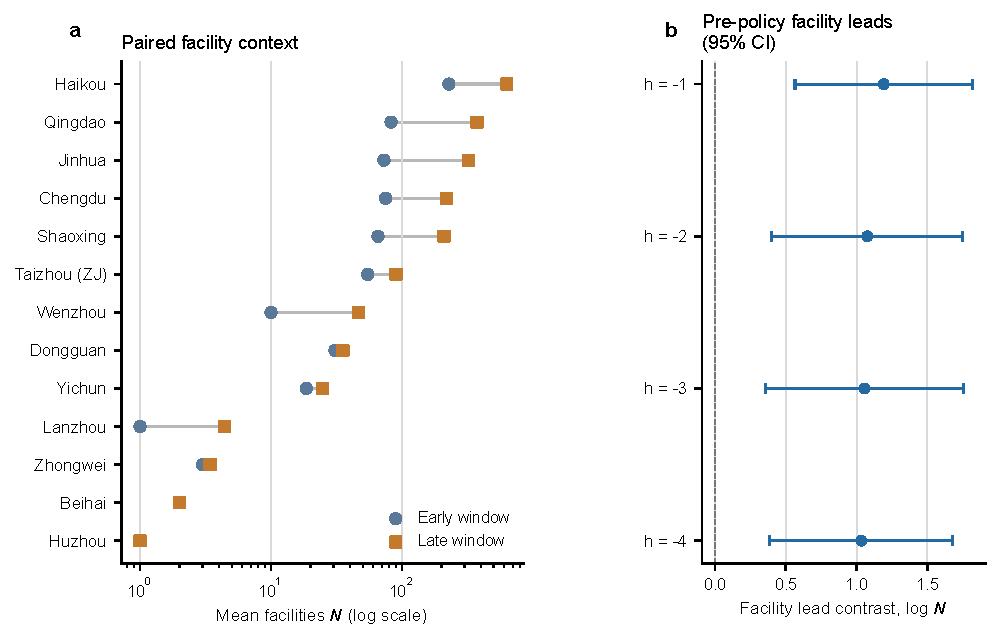
\includegraphics[width=\linewidth,height=.76\textheight,keepaspectratio]{figures/figS_governance.pdf}
\caption{Facility context and governance comparison}\label{fig:si_governance}
\end{figure}
\FloatBarrier

Table~\ref{tab:responses} retains the first-year, common-eight-city,
second-year, time, city-composition and total contrasts with their support
counts and joint intervals.  The independent pre-policy coefficients are in
Table~\ref{tab:leads}; their $p=0.0008415$ facility test is a support diagnostic
and is not subtracted from the post-policy target.  Figure~\ref{fig:si_windows}
separates the common-eight-city first/second-year estimates from those window
decomposition terms, so the distinct reference structures remain visible.
\begin{table}[htbp]
\centering\small
\caption{Window response contrasts}\label{tab:responses}
\begin{tabular}{p{.27\linewidth}rrr}
\toprule
Target & $\ln A$ & $\ln N$ & $\delta$ \\
\midrule
First year (11 cities) & 1.790 [-0.135, 3.286] & 0.701 [0.081, 1.251] & 1.089 [-0.920, 2.766] \\
First year, common cities (8) & 2.377 [0.029, 4.162] & 0.674 [-0.032, 1.368] & 1.703 [-0.912, 3.696] \\
Second year, common cities (8) & 4.063 [1.675, 6.248] & 1.184 [0.342, 2.142] & 2.879 [0.366, 5.382] \\
Second minus first year & 1.687 [0.083, 3.470] & 0.511 [0.107, 1.011] & 1.176 [-0.115, 2.691] \\
City-composition term & 0.587 [-0.111, 1.677] & -0.027 [-0.352, 0.345] & 0.614 [-0.104, 1.739] \\
Total window gap & 2.274 [0.628, 4.088] & 0.483 [-0.003, 1.067] & 1.790 [0.380, 3.461] \\
First year, pre-supported (8) & 1.532 [0.109, 2.707] & 0.688 [0.085, 1.172] & 0.843 [-0.340, 1.891] \\
Pre-supported minus full set & -0.258 [-1.515, 1.028] & -0.013 [-0.409, 0.363] & -0.246 [-1.781, 1.377] \\
\bottomrule
\end{tabular}
\end{table}

\begin{table}[htbp]
\centering\small
\caption{Pre-policy lead coefficients}\label{tab:leads}
\begin{tabular}{rrrrr}
\toprule
$h$ & Cities & $\ln A$ & $\ln N$ & Derived $\delta$ \\
\midrule
-4 & 7 & 0.501 [-1.267, 2.269] & 1.033 [0.385, 1.680] & -0.532 [-2.192, 1.129] \\
-3 & 8 & 0.780 [-1.132, 2.692] & 1.054 [0.356, 1.752] & -0.274 [-1.973, 1.425] \\
-2 & 8 & 1.221 [-0.340, 2.781] & 1.075 [0.401, 1.749] & 0.146 [-1.115, 1.407] \\
-1 & 10 & 2.042 [-0.144, 4.228] & 1.191 [0.565, 1.818] & 0.851 [-1.010, 2.712] \\
\bottomrule
\end{tabular}
\end{table}

\FloatBarrier
\begin{figure}[htbp]\centering
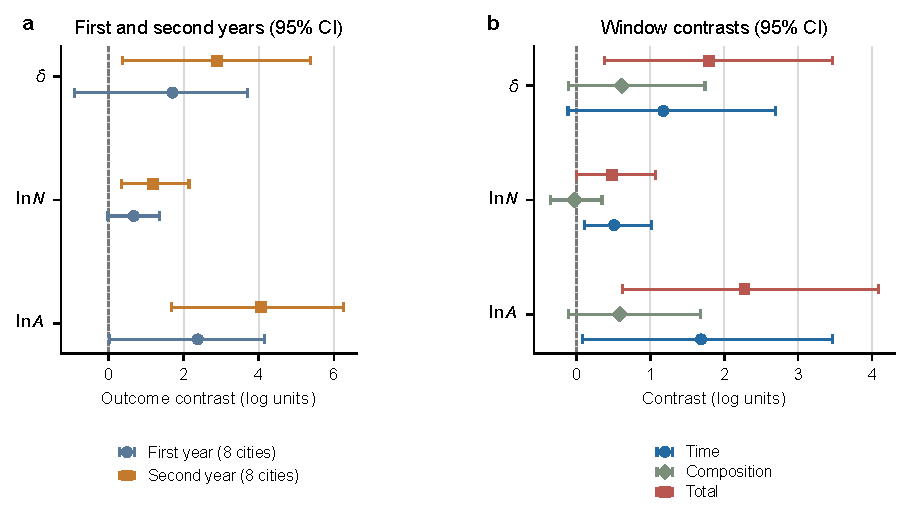
\includegraphics[width=.92\linewidth]{figures/figS_window_decomposition.pdf}
\caption{First- and second-year comparisons}\label{fig:si_windows}
\end{figure}
\FloatBarrier

The first-/second-year comparison therefore separates the common-eight-city
time term from the city-composition term and total gap in Table~\ref{tab:responses}.
The complete target-specific bootstrap intervals and lead supports remain
separate, rather than being combined into one event-time estimate.

For intensity, the total window gap is 1.790 log units with 95\% CI
$[0.380,3.461]$, whereas the same-city second-minus-first-year time term is
1.176 with CI $[-0.115,2.691]$.  The overall cross-window difference therefore
has a positive interval even though the matched-city time component is
compatible with zero; city composition and the distinct reference structures
contribute to the total contrast.

\section{City trajectories and observation coverage}
\label{sec:si-trajectories}
The 11-city governance target has 160 city-quarters in its full observation
window.  Eight city-quarters have no compatible weeks and therefore have
missing outcome ratios; lines break at these missing observations rather than
interpolating across them.  A source-coded-zero share is the fraction of
compatible weekly records coded zero, not a verified zero-transaction rate.
Block summaries average defined quarterly ratios within their city-quarter
support rather than pooling weekly records.  The three panels retain the
outcome variables, calendar ordering, missing segments and observation-state
coding used by the governance comparison.

Figures~\ref{fig:si_city_paths_1}, \ref{fig:si_city_paths_2} and
\ref{fig:si_city_paths_3} provide the city-level check on the aggregate
governance contrasts: each page aligns $A$, $N$, $I$ and observation status on
the same relative-time axis.  Circles mark the three outcome series; in the
observation column, black circles denote time coverage and orange squares the
source-coded-zero share.  Grey shading marks a policy-transition quarter and
the dashed vertical line marks $h=0$; missing city-quarters break the lines.
These event markers orient the comparison but do not assign observed changes to
a policy.

The plotted trajectories also show why a window average can combine different
level and timing patterns.  For Haikou, $A$ rises from about 47,642 at $h=-8$
to 176,178 at $h=0$ while $N$ rises from 84.7 to 810.1 and $I$ falls from
562.5 to 217.5.  Fuzhou has missing outcome ratios at $h=-7$ and $h=-6$;
after complete coverage resumes, $A$ remains near 1,200 through $h=3$ before
reaching 13,724 at $h=4$, while $I$ rises from 46.2 at $h=0$ to 303.4 at
$h=4$.  These are descriptive city paths, not policy-effect estimates.

\clearpage\begin{center}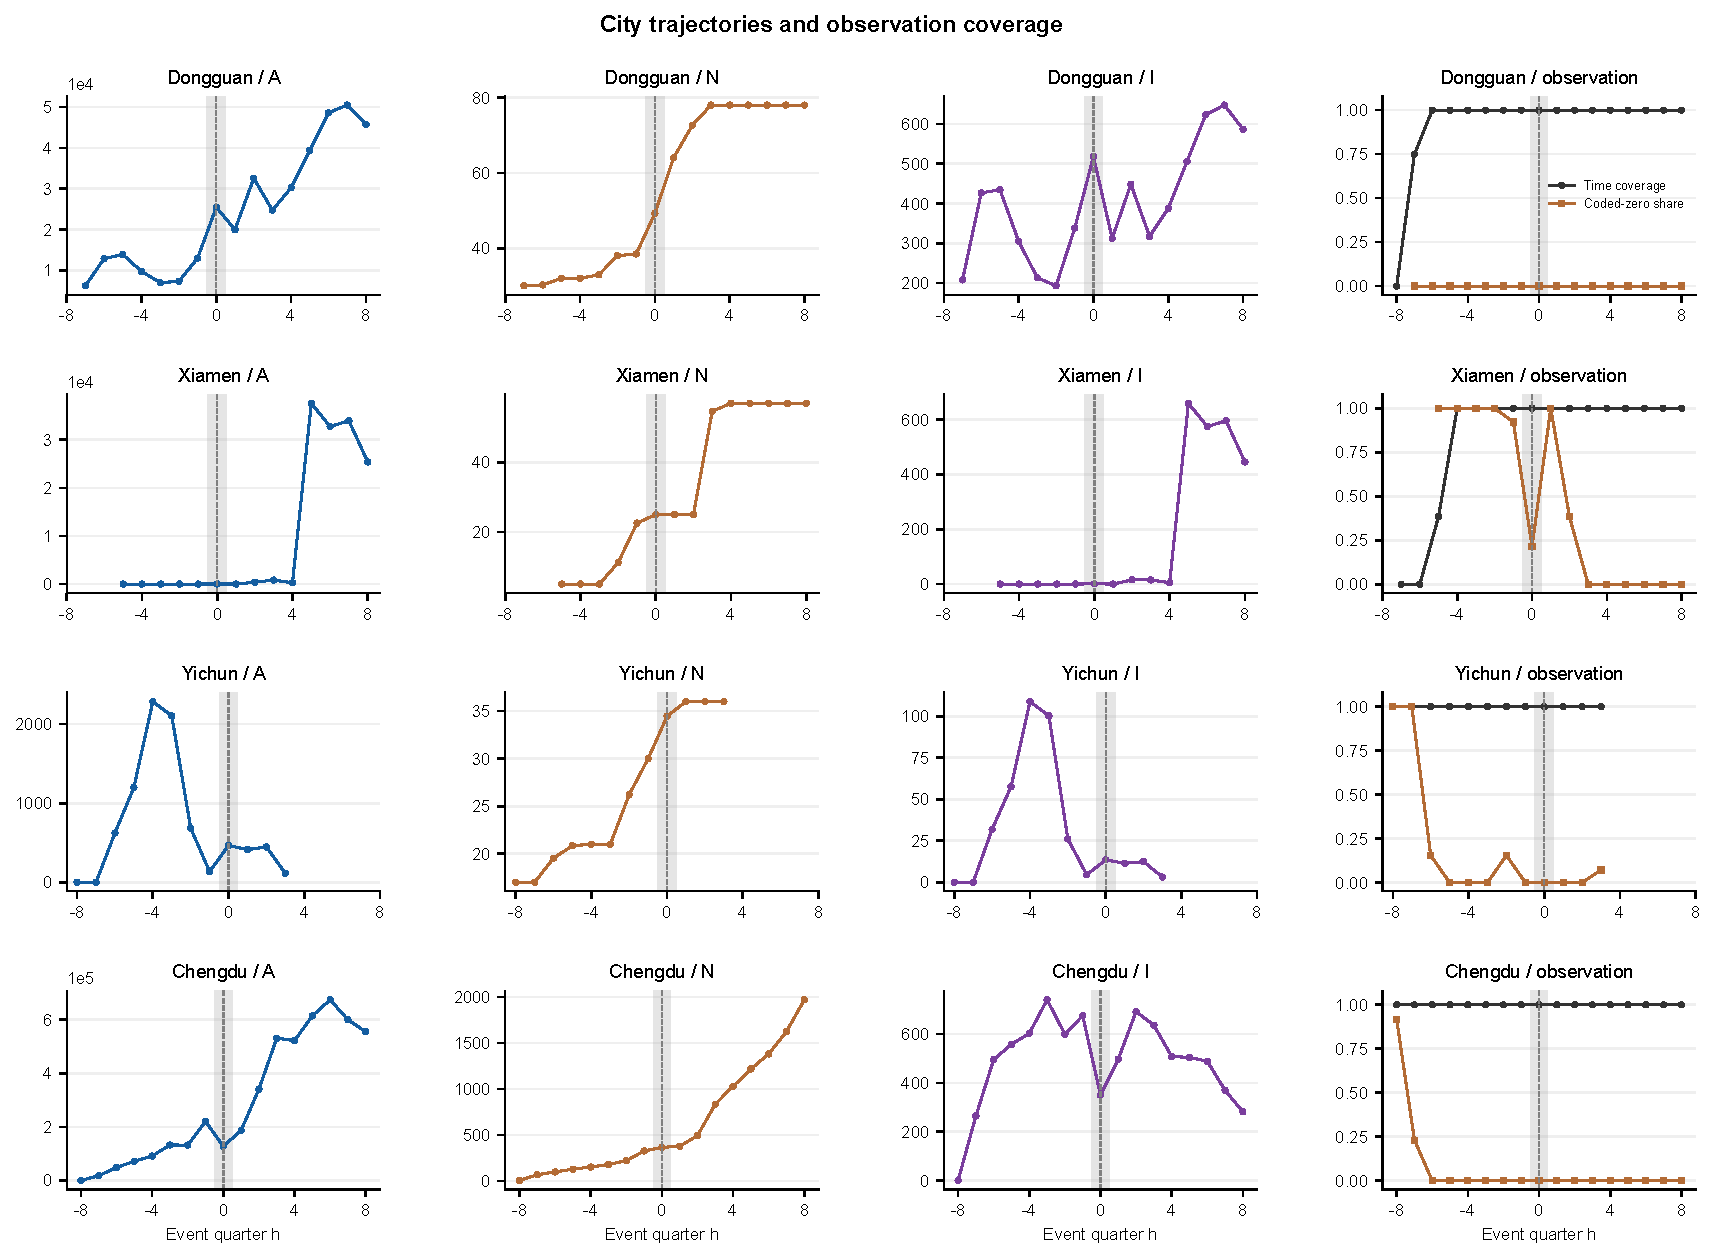
\includegraphics[width=\linewidth,height=.78\textheight,keepaspectratio]{figures/figS_city_paths_1.pdf}\captionof{figure}{City outcome paths and observation states, group 1}\label{fig:si_city_paths_1}\end{center}
\clearpage\begin{center}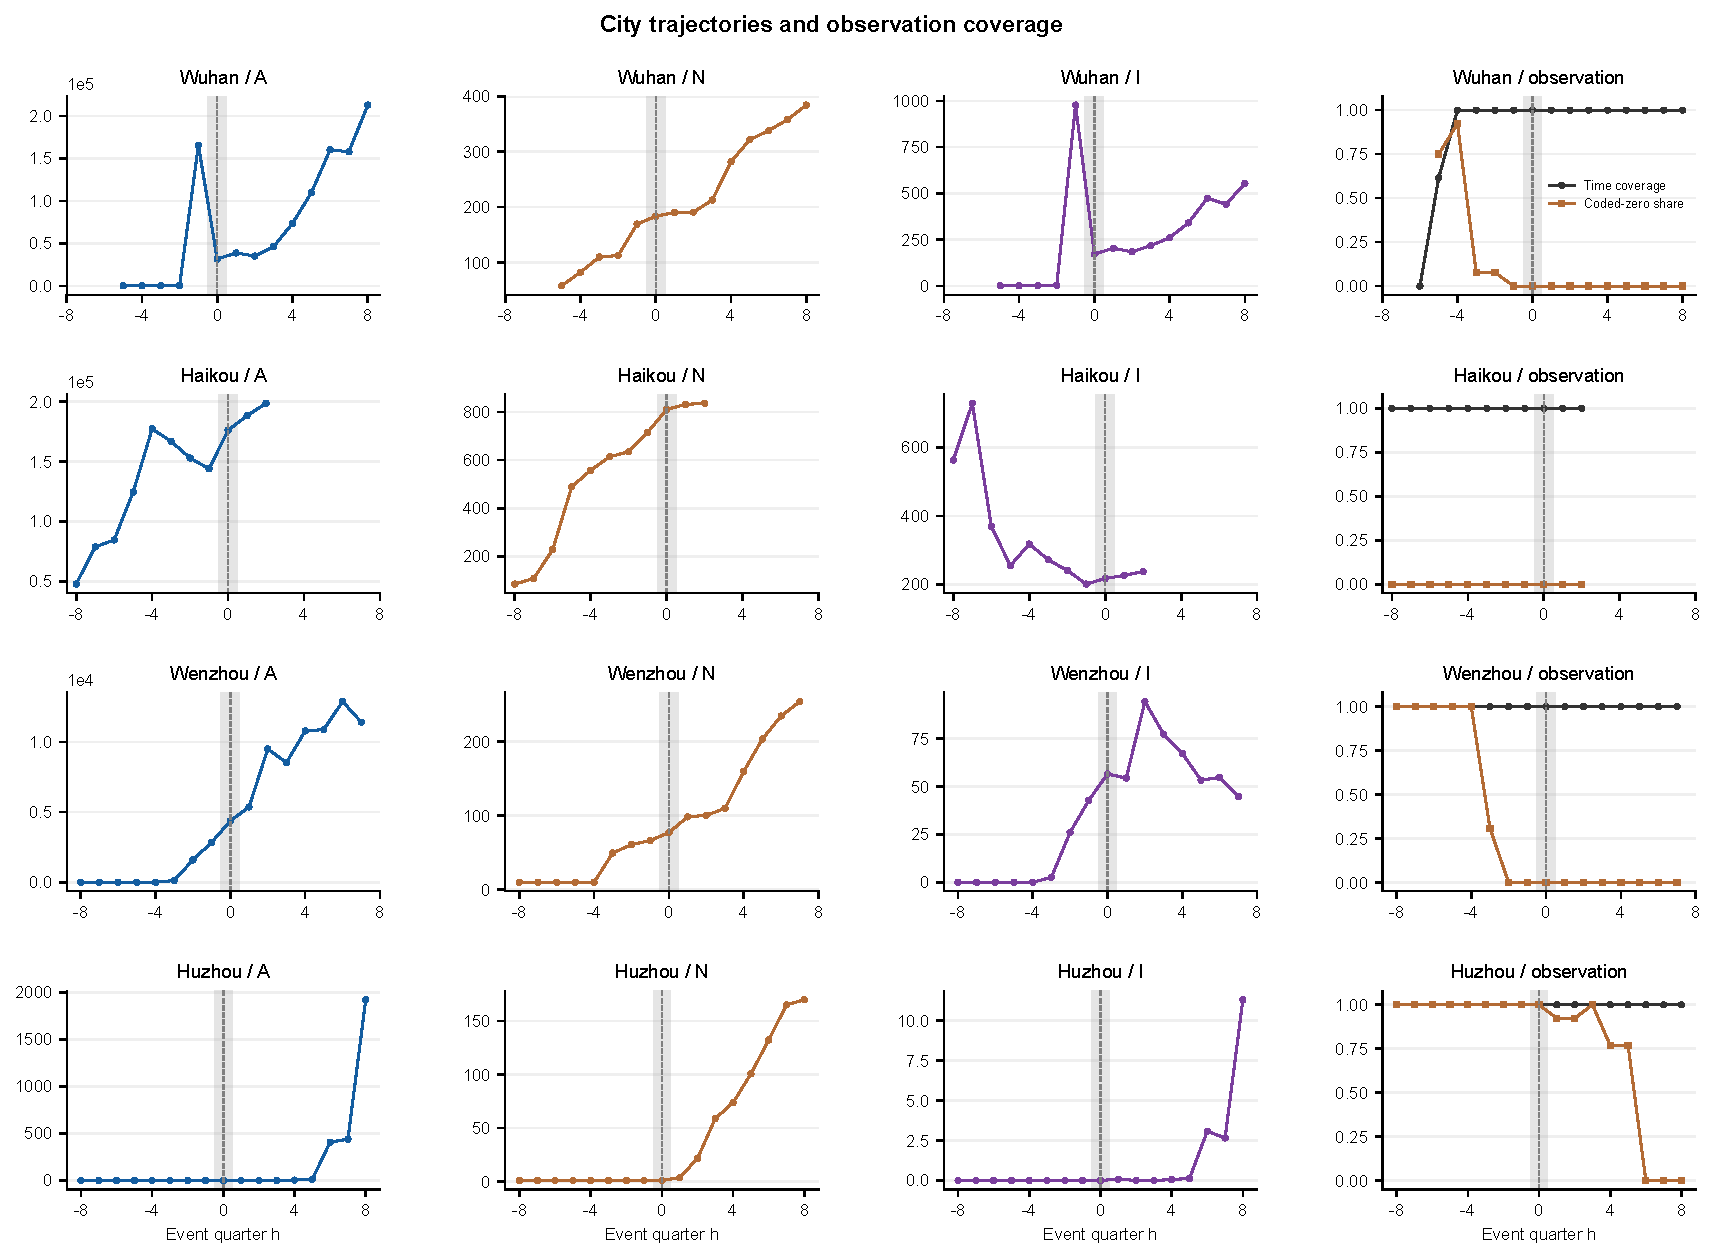
\includegraphics[width=\linewidth,height=.78\textheight,keepaspectratio]{figures/figS_city_paths_2.pdf}\captionof{figure}{City outcome paths and observation states, group 2}\label{fig:si_city_paths_2}\end{center}
\clearpage\begin{center}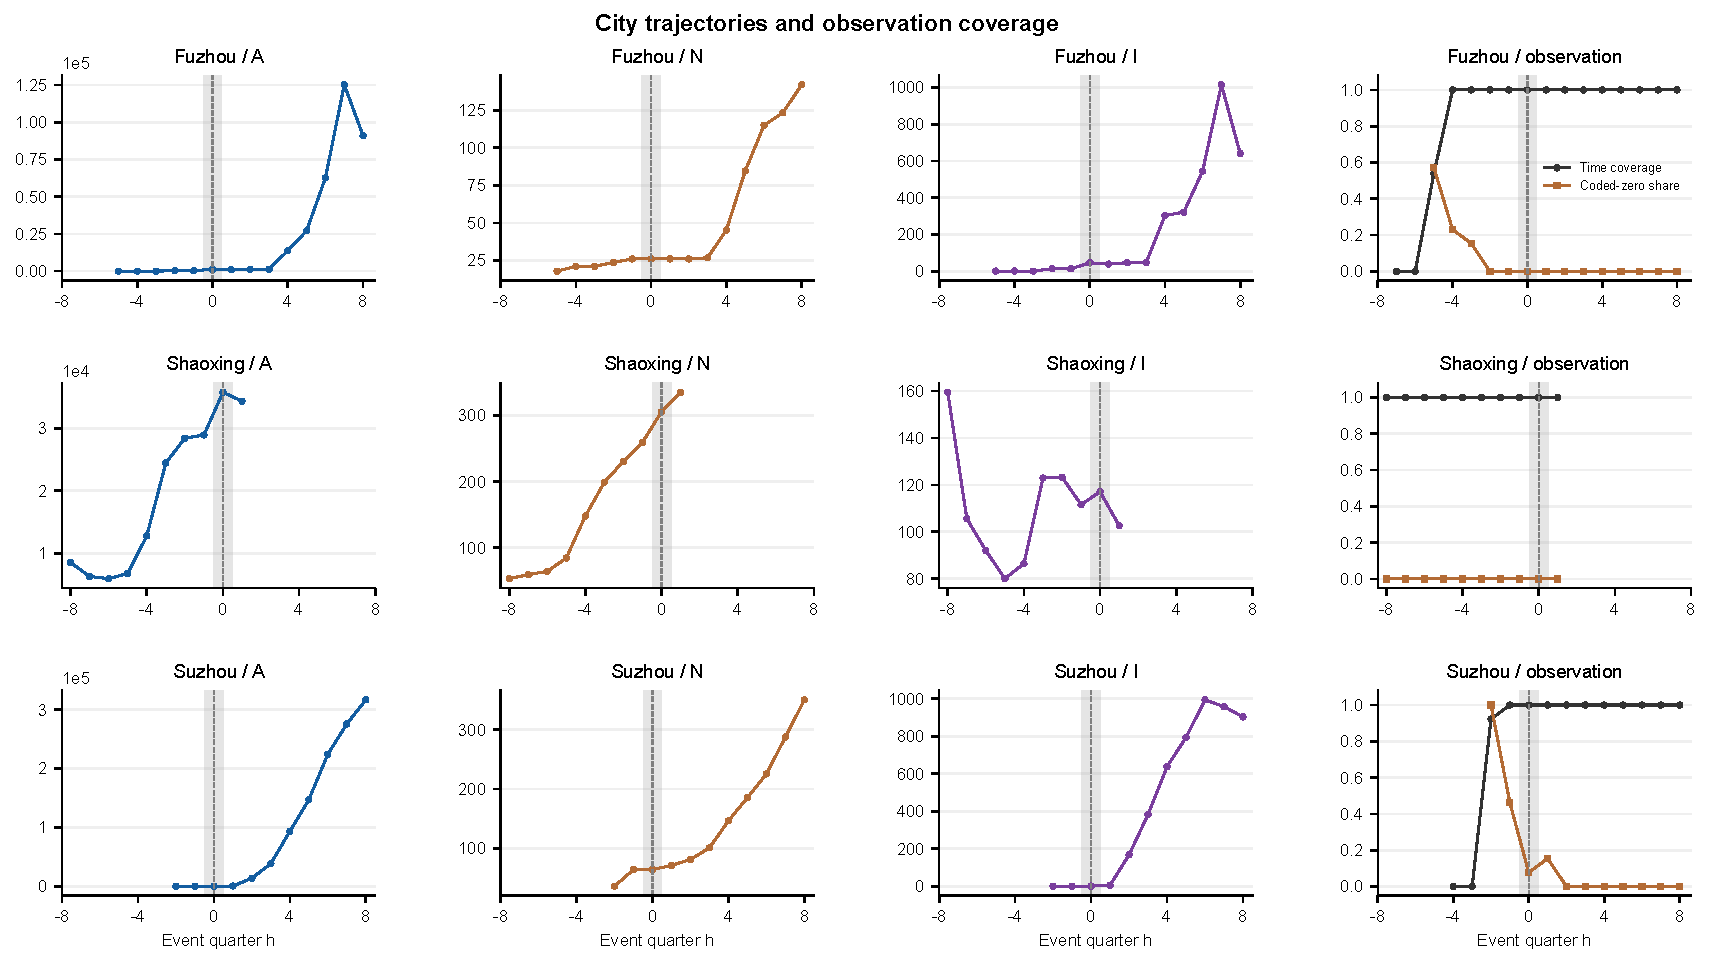
\includegraphics[width=\linewidth,height=.78\textheight,keepaspectratio]{figures/figS_city_paths_3.pdf}\captionof{figure}{City outcome paths and observation states, group 3}\label{fig:si_city_paths_3}\end{center}

